% BEGIN PREAMBEL
\documentclass[9pt]{beamer}
\usepackage[british]{babel}
\usepackage[latin1]{inputenc}
\usepackage{amsmath,amsfonts,amssymb}
\usepackage{upgreek}
\usepackage{pgfpages}
\usepackage[version=3]{mhchem}
\usepackage{lmodern}
\usepackage{graphicx}
\usepackage{multicol}
\usepackage{xcolor}
\usepackage{wrapfig}
\newcommand{\as}{\\[14pt]}
\newcommand{\s}{\\[7pt]}
\newcommand{\is}{\\[2pt]}
\newcommand{\no}{\noindent}
\newcommand{\ka}{\hspace*{0.5cm}}
\newcommand{\ma}{\hspace*{1cm}}
\newcommand{\ga}{\hspace*{1.5cm}}
\newcommand{\li}{\left|}
\newcommand{\re}{\right|}
\newcommand{\const}{\text{const.}}
\newcommand{\z}{\text}
\newcommand{\terminal}[1]{\colorbox{black}{\textcolor{white}{{\fontfamily{phv}\selectfont \scriptsize{#1}}}}}
\newcommand{\plugin}[1]{\textit{\flq#1\frq}}
\usetheme{Boadilla}
\usecolortheme{beaver}
\useoutertheme{miniframes}
\graphicspath{ {Pics/} }
\beamertemplatenavigationsymbolsempty
\makeindex
\title[ETH High Rate Beam Telescope]{ETH High Rate Beam Telescope}
\author[M. Reichmann]{Michael Reichmann}
\institute[\textbf{\textit{ETH}}\scalebox{.6}{\textit{Z\"{u}rich}}]{Swiss Federal Institute of Technology Zurich}
% END PREAMBEL
\begin{document}
% ============================
% BEGIN TITLE PAGE
% ============================
\begin{frame}
	\begin{center}
		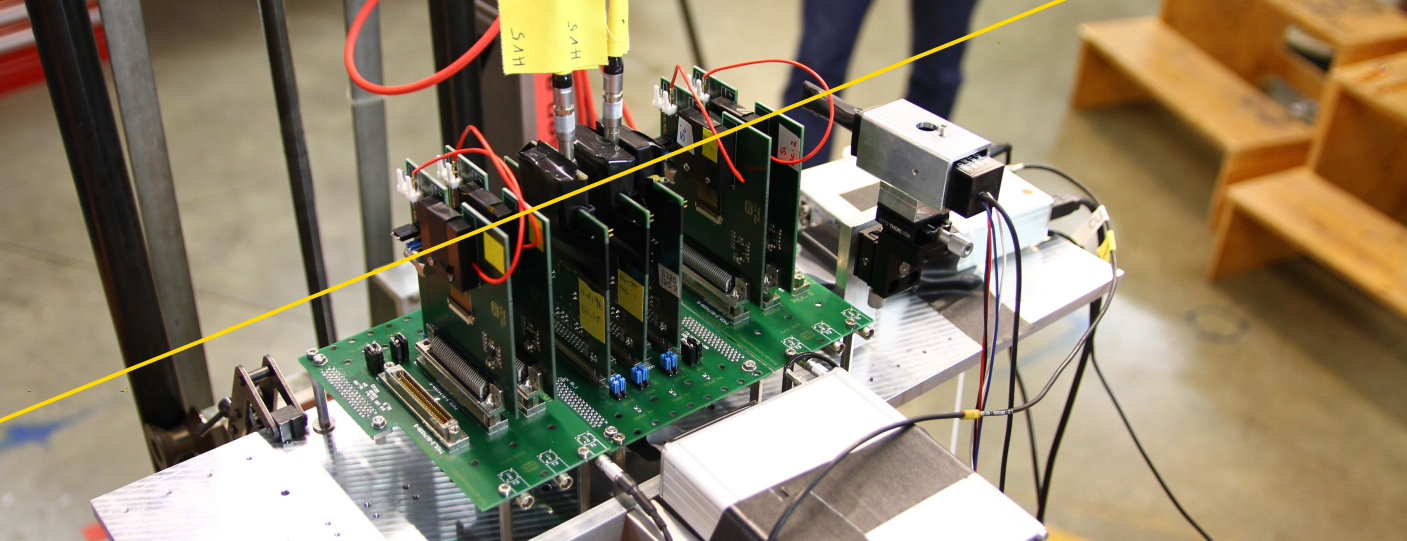
\includegraphics[width=10cm]{Pics/telescope1}
	\end{center}
	\begin{alertblock}{
		\begin{center}
			\textbf{ETH High Rate Beam Telescope}
		\end{center}}
		\vspace*{10pt}
		\begin{center}\small
			presented by: Michael Reichmann \\ 
			coauthors: Felix Bachmair, Dmitry Hits
		\end{center}\normalsize
	\end{alertblock}
\end{frame}
% ============================
% TABLE OF CONTENTS
% ============================
\begin{frame}%[allowframebreaks]
	\frametitle{Table of contents}
	\tableofcontents[hideallsubsections]   % [pausesections]
\end{frame}
% END
% ====================================================================================
% BEGIN MOTIVATION
% ====================================================================================
\section{Motivation}
\begin{frame}
	\begin{alertblock}{
		\begin{center}
			\Large{\textbf{Motivation}}
		\end{center}}
	\end{alertblock}
\end{frame}
% new frame ============================
\begin{frame}
	\underline{\textbf{Goal:}}
	\begin{itemize}
		\item testing of different types of diamond sensors for rate dependence (up to fluxes of $10\,\z{MHz/cm}^{2}$)
	\end{itemize}
	\underline{\textbf{Conditions:}}
	\begin{itemize}
		\item beam line PIM1 at PSI (Paul Scherrer institute)
		\item continous pion beam with a flux of up to $10\,\z{MHz/cm}^{2}$ and momenta of $100$-$500$\,MeV/c
	\end{itemize}
	\underline{\textbf{Requirements:}}
	\begin{itemize}
		\item small, flexible and modular system
		\begin{itemize}
			\item reduce effects of multiple scattering
			\item fast setup, easy to tear down, 
		\end{itemize}
		\item high rate continuous data taking
		\item scalable trigger area
		\begin{itemize}
			\item high efficiency in the DUT
		\end{itemize}
		\item precise trigger timing
	\end{itemize}
\end{frame}
% END
% ====================================================================================
% BEGIN TELESCOPE
% ====================================================================================
\section{The Telescope}
\begin{frame}
	\begin{alertblock}{
		\begin{center}
			\Large{\textbf{The Telescope}}
		\end{center}}
	\end{alertblock}
	\begin{center}
		\begin{minipage}{5.5cm}
			\centering
			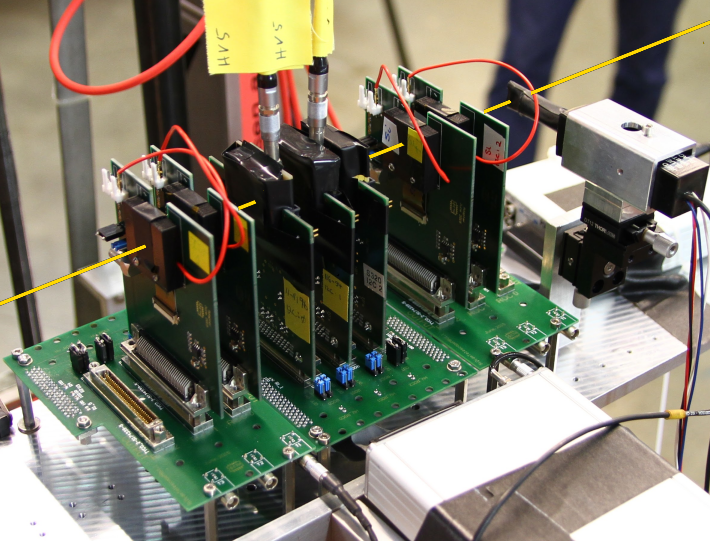
\includegraphics[height=4.5cm]{Pics/telescope2}
		\end{minipage}
		\hspace*{2pt}
		\begin{minipage}{5.5cm}
			\centering
			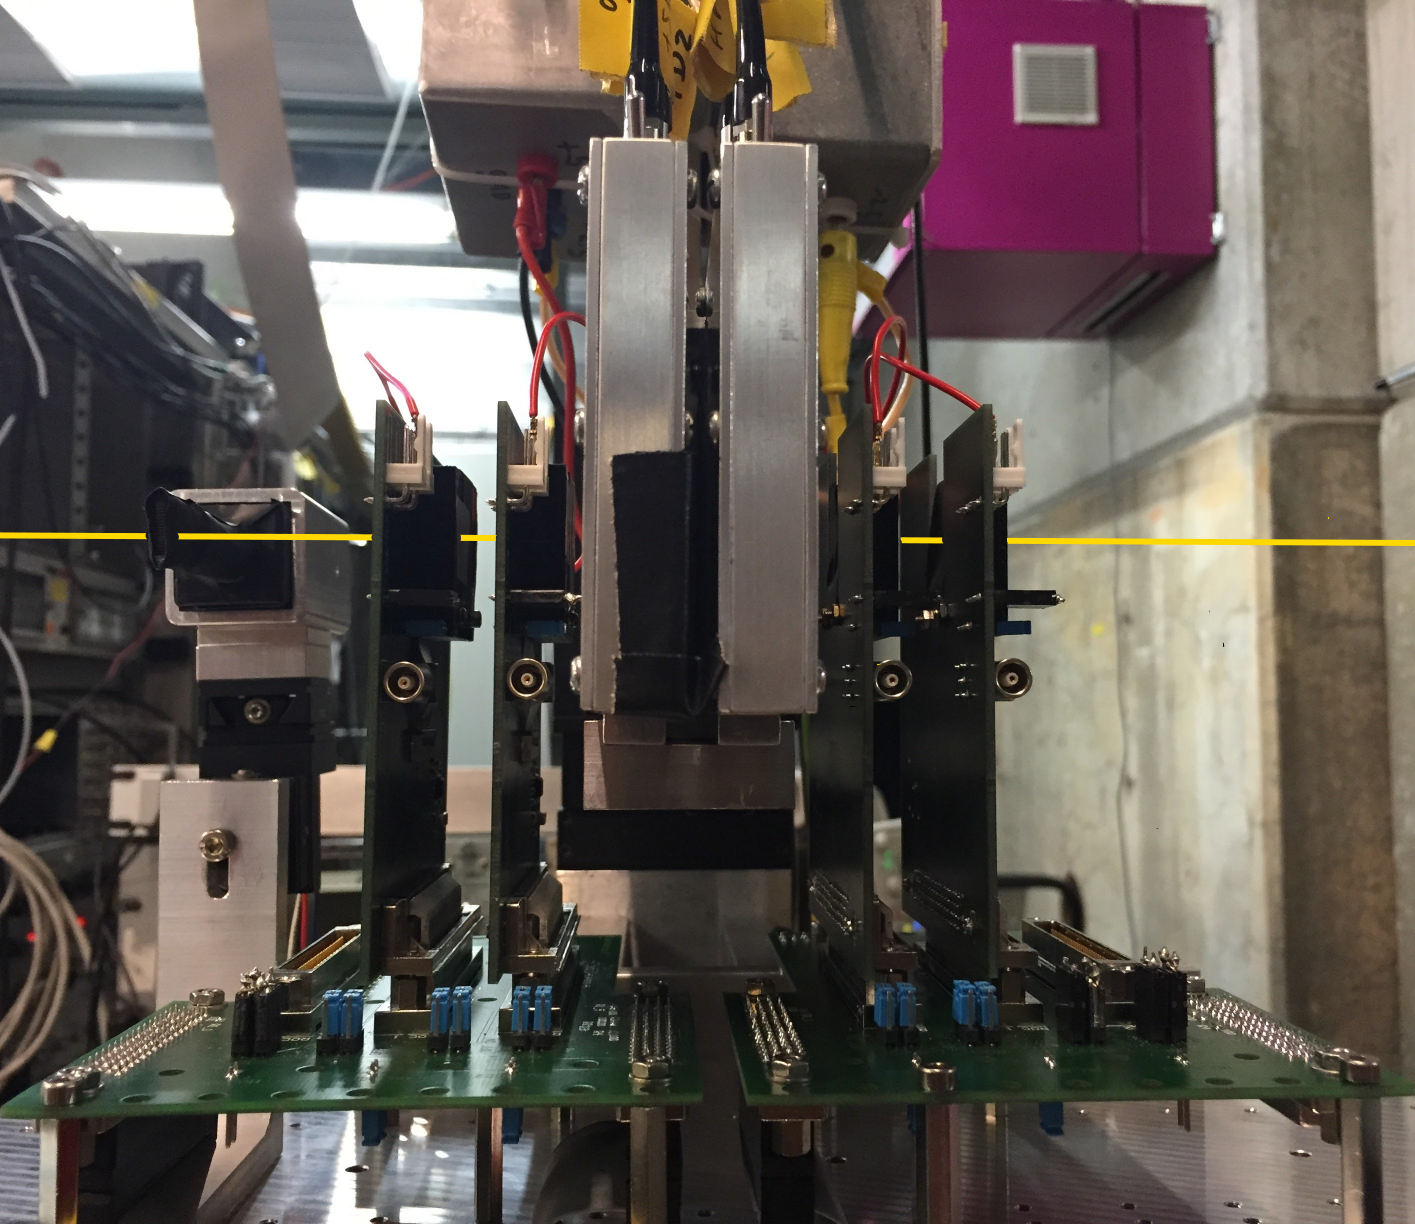
\includegraphics[height=4.5cm]{Pics/telescope3}
		\end{minipage}
	\end{center}
\end{frame}
% ============================
% GENERAL SETUP
\subsection{Telescope Module}
\begin{frame}
	\frametitle{Telescope Module}
	\begin{center}
		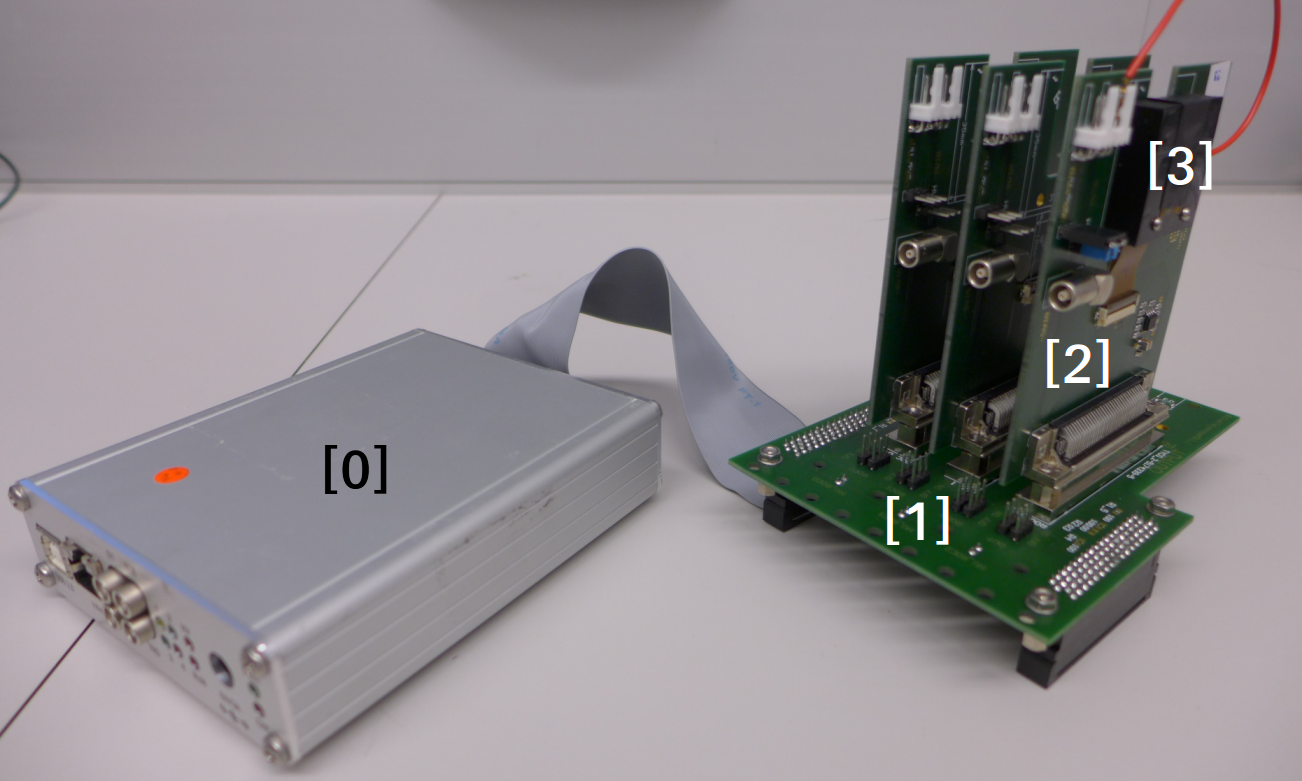
\includegraphics[width=7.8cm]{Pics/setup}
	\end{center}
	\begin{itemize}
		\item $[0]$ DTB (Digital Test Board): interface to a computer
		\item $[1]$ Motherboard: main frame of the telescope
		\item $[2]$ Adapter Planes: interface to the single pixel chips
		\item $[3]$ CMS Pixel Chip (analogue or digital)
	\end{itemize}
\end{frame}
% ============================
% CHIP OVERVIEW
\subsection{Parts}
\setlength\extrarowheight{5pt}
\begin{frame}
	\frametitle{CMS Pixel Chips}
	\begin{table}[ht]
		\centering
		\begin{tabularx}{.95\textwidth}{Xlll}
									&\textbf{PSI46v2}					&\textbf{PSI46dig}					&\textbf{PROC600}					\\\noalign{\hrule height 2pt}
			Chip size				&\multicolumn{3}{c}{$\approx 8\times10$\,mm$^{2}$}															\\\hline
% 			Chip size				&$7.9 \times 10.0$\,mm$^{2}$		&$7.9 \times 10.3$\,mm$^{2}$		&$7.9 \times 10.6$\,mm$^{2}$		\\\hline
			Pixel size				&\multicolumn{3}{c}{$150 \times 100$\,$\upmu$m$^{2}$}														\\\hline
% 			Pixel size				&$150 \times 100$\,$\upmu$m$^{2}$	&$150 \times 100$\,$\upmu$m$^{2}$	&$150 \times 100$\,$\upmu$m$^{2}$	\\\hline
			Pixel array				&\multicolumn{3}{c}{$52 \times 80$}																			\\\hline
% 			Pixel array				&$52 \times 80$						&$52 \times 80$						&$52 \times 80$						\\\hline
			\textbf{Pixel charge readout}	&\textbf{analogue}			&\textbf{digitised}					&d\textbf{igitised}					\\\hline
			Readout					&multi level \@ $40$\,MHz			&$160$\,MBit/sec					&$160$\,MBit/sec					\\\hline
			Hit rate				&$80$\,MHz/cm$^{2}$					&$120$\,MHz/cm$^{2}$				&$600$\,MHz/cm$^{2}$				\\\hline
			Radiation Tolerance		&$200$\,kGy							&$1$\,MGy							&$6$\,MGy (exp.)					\\\hline
			\textbf{In-time threshold}		&$\mathbf{3500}$\,\textbf{e}&$\mathbf{\approx1500}$\,\textbf{e}	&$\mathbf{\approx1500}$\,\textbf{e}	\\\hline
			\textbf{Fast-OR trigger}&\textbf{yes}						&\textbf{no}						&\textbf{yes}						\\\hline
		\end{tabularx}
	\end{table}
\end{frame}
% ============================
% PARTS
\subsection{Parts}
\begin{frame}
	\begin{center}
		\begin{minipage}{5.5cm}
			\centering
			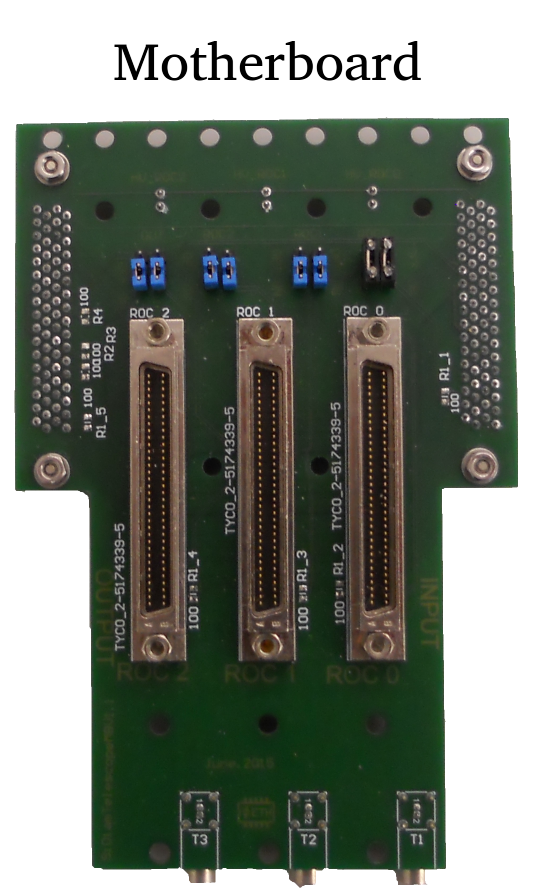
\includegraphics[height=6cm]{Pics/Motherboard1}
		\end{minipage}
		\hspace*{2pt}
		\begin{minipage}{5.5cm}
			\centering
			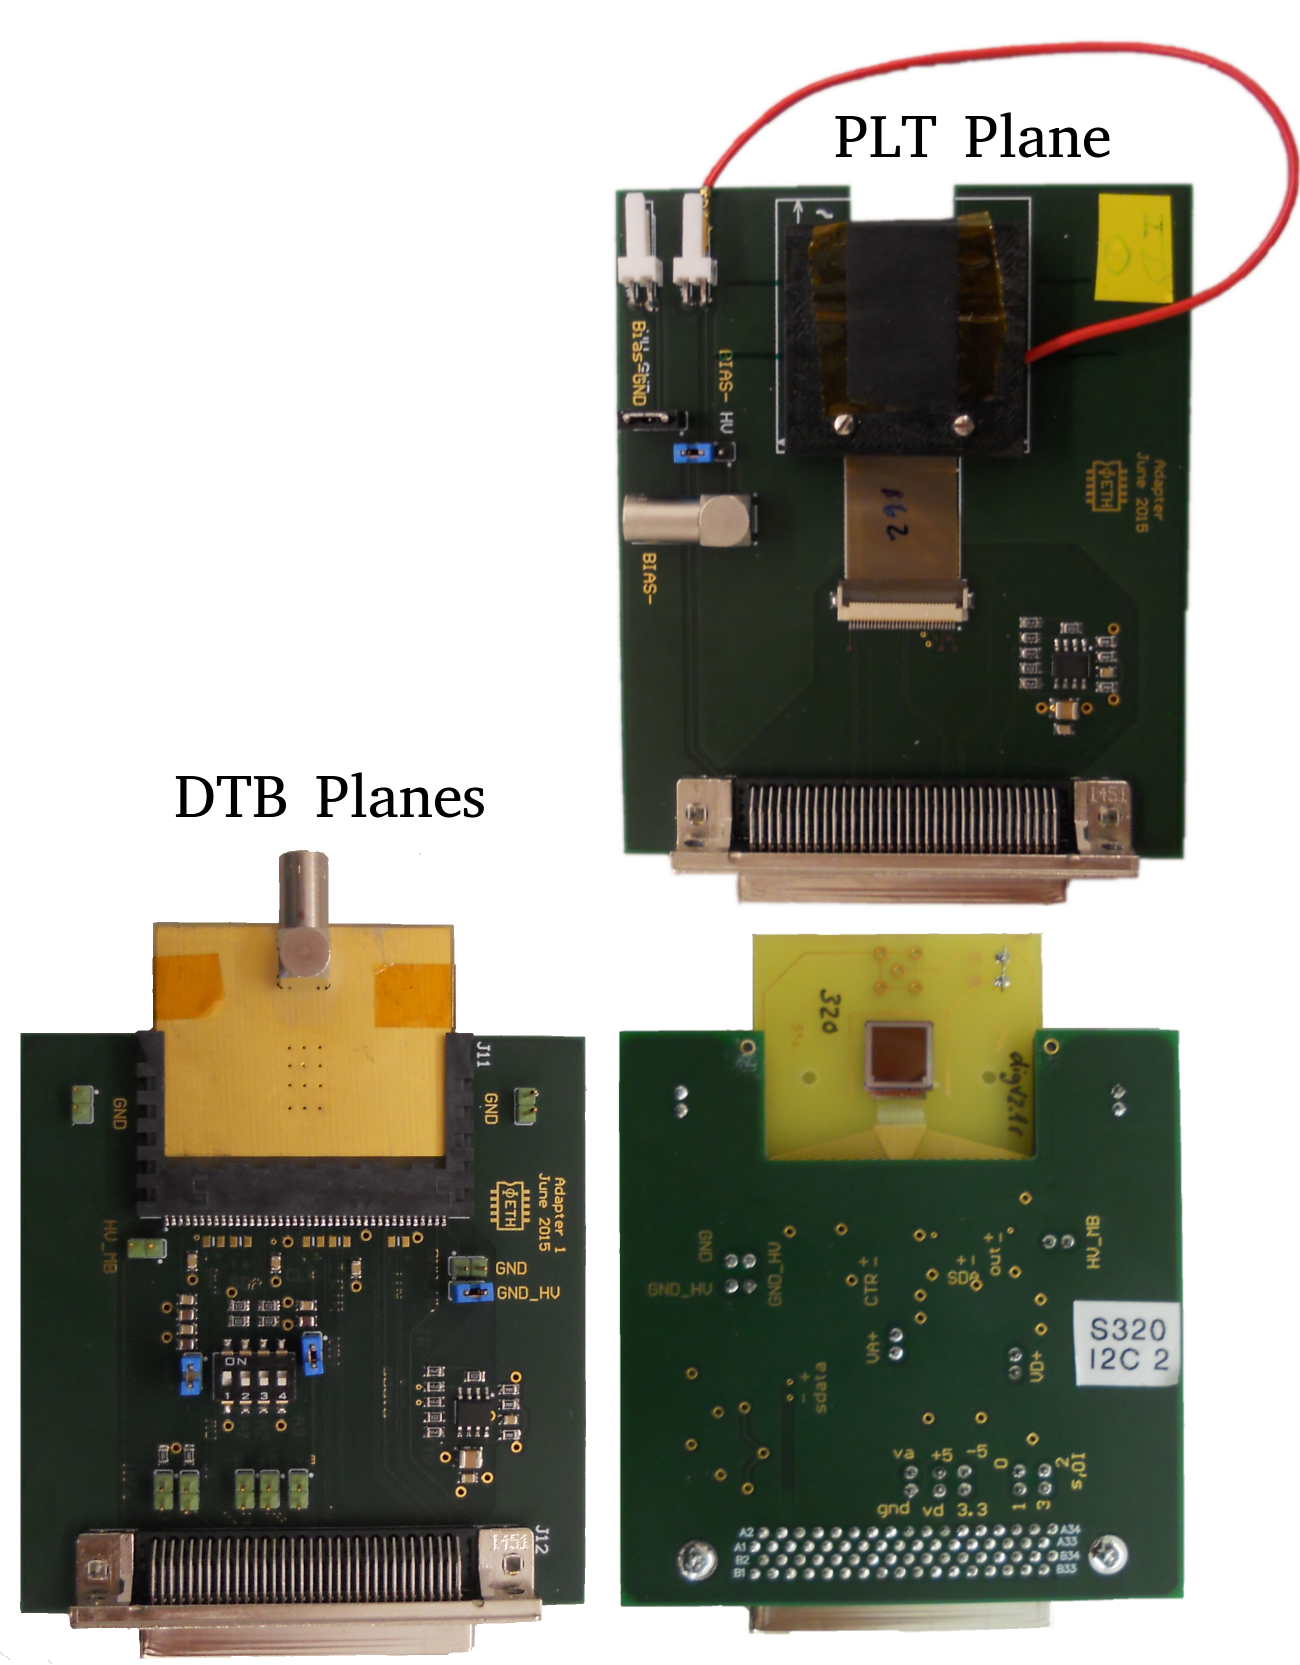
\includegraphics[height=7cm]{Pics/Adapters}
		\end{minipage}
	\end{center}
\end{frame}
% ============================
% SETUP
\subsection{Setups}
\begin{frame}
	\frametitle{Schematic Setup}
	\begin{center}
		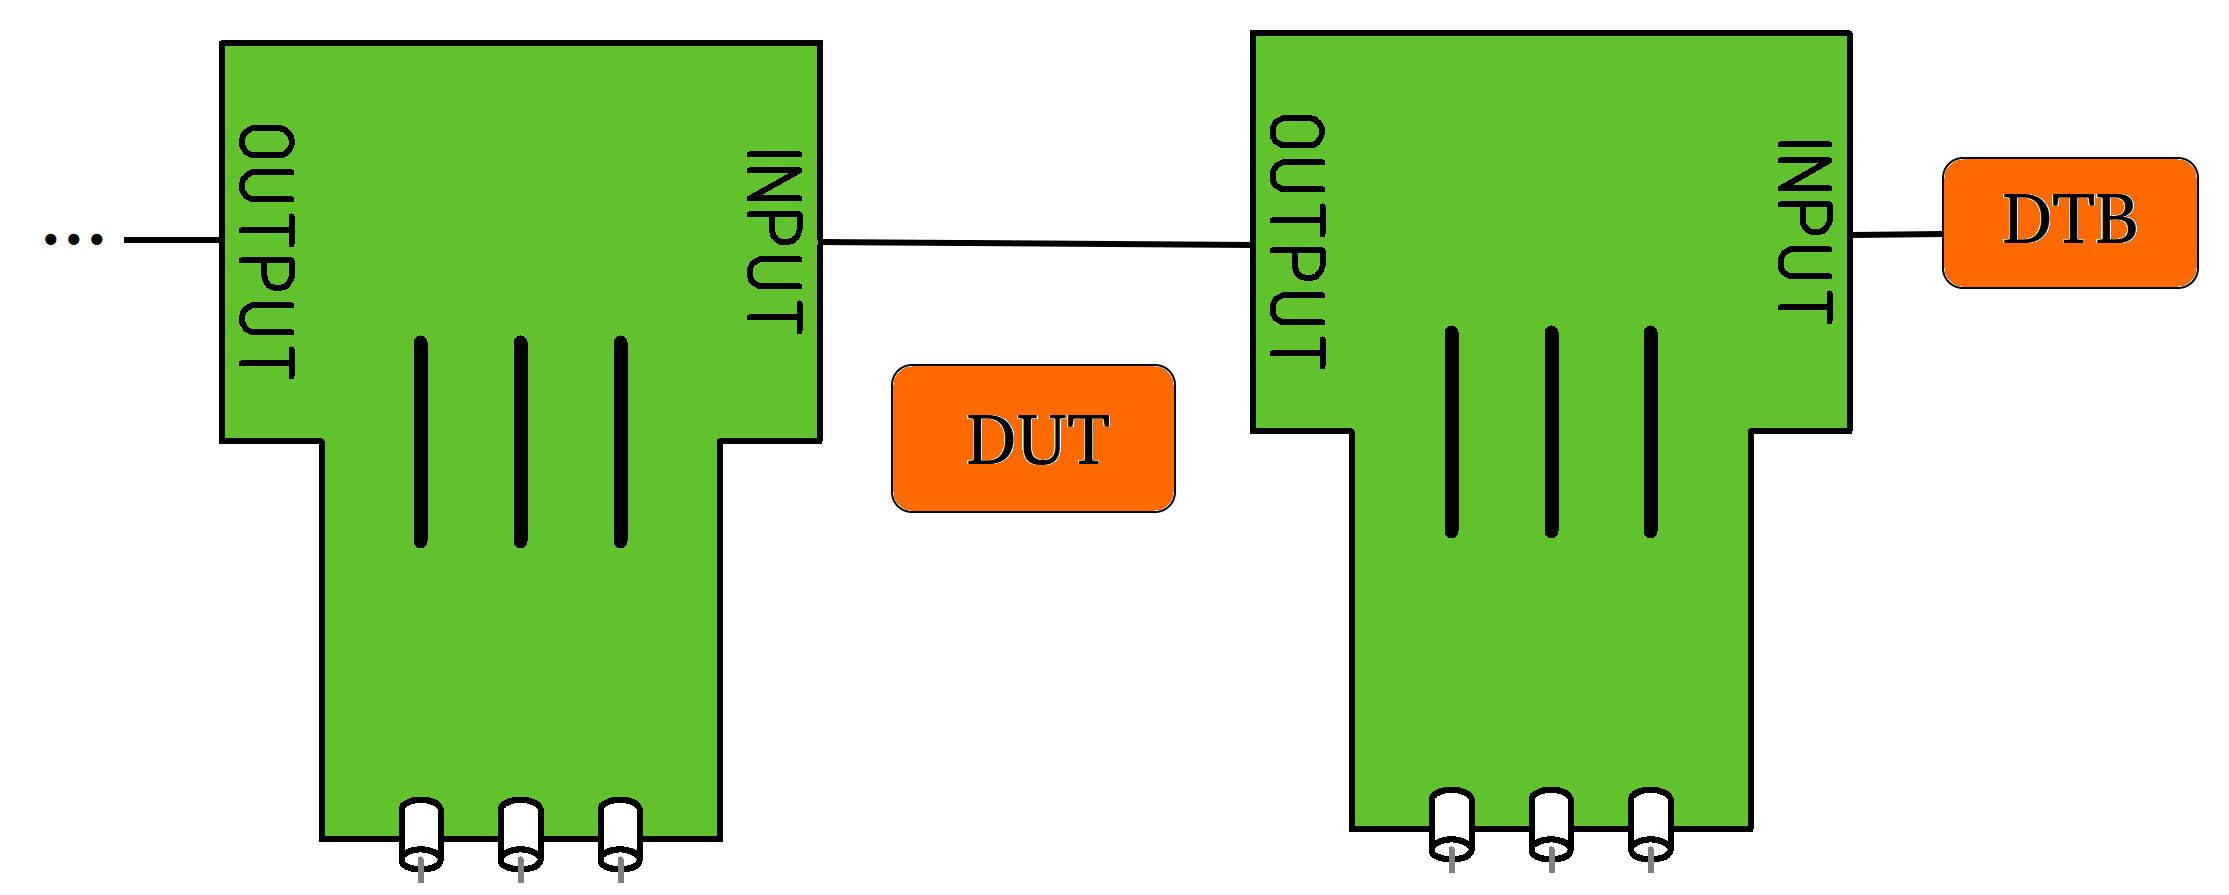
\includegraphics[width=8cm]{Modul}
	\end{center}
	\begin{itemize}
		\item chain several motherboards together into a single big telescope
		\item can only chain one chip type (analogue or digital)
		\item number of planes per motherboard is also variable ($1-3$)
	\end{itemize}
\end{frame}
% new frame ============================
\begin{frame}
	\frametitle{Diamond Pixel Setup}
	\begin{center}
		\begin{minipage}{4cm}
			\centering
			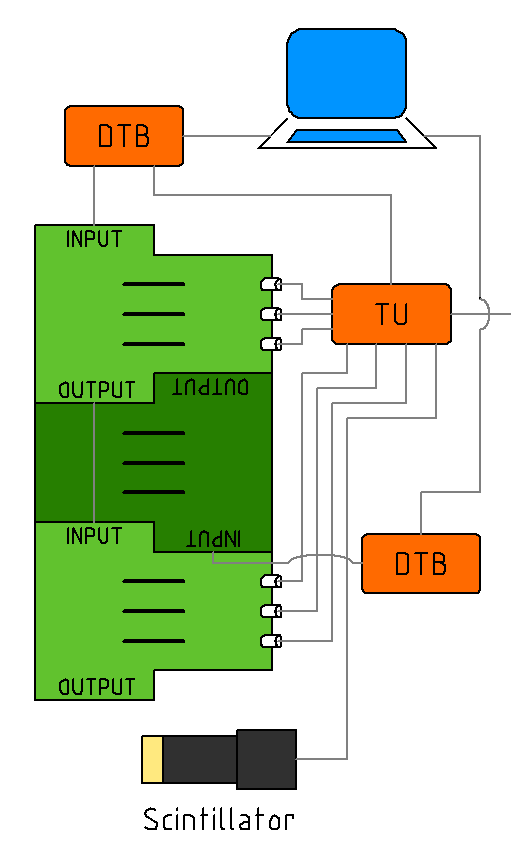
\includegraphics[width=4cm]{fulltel_scint}
		\end{minipage}
% 		\hspace*{2pt}
		\only<1>{
		\hspace*{1pt}
			\begin{minipage}[c][.7\textheight]{7cm}
				\begin{itemize}
					\setlength{\itemsep}{\fill}
					\item telescope: two motherboards
					\begin{itemize}
						\item analogue chips 
					\end{itemize}
					\item DUT: single motherboard
					\begin{itemize}
						\item diamonds sensors on digital chips
					\end{itemize}
					\item scintillator: precise trigger timing  (fast-OR depends on clock, usually $40$\,MHz)
					\item trigger: coincidence of the two planes closest to the DUT (red) and the scintillator
				\end{itemize}
			\end{minipage}}
		\only<2>{
			\begin{minipage}{7cm}
				\centering
				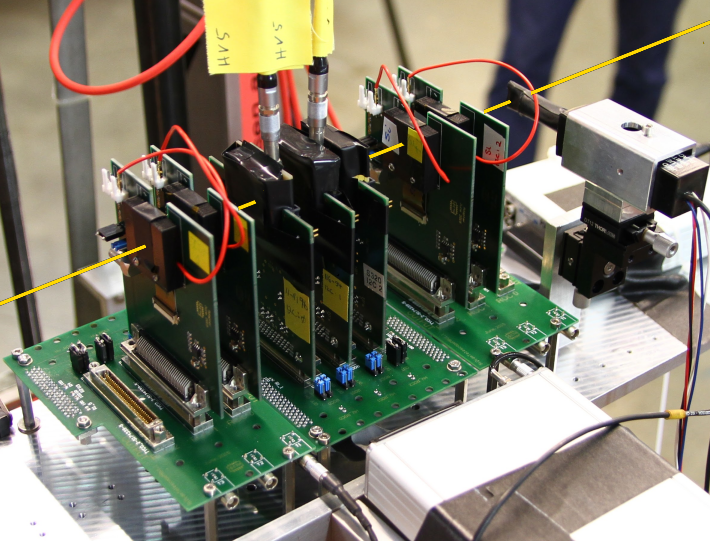
\includegraphics[width=6cm]{Pics/telescope2}
			\end{minipage}}
	\end{center}
\end{frame}
% new frame ============================
\setlength\extrarowheight{5pt}
\begin{frame}
	\frametitle{Specification}
	\begin{center}
		\begin{minipage}{4cm}
			\centering
			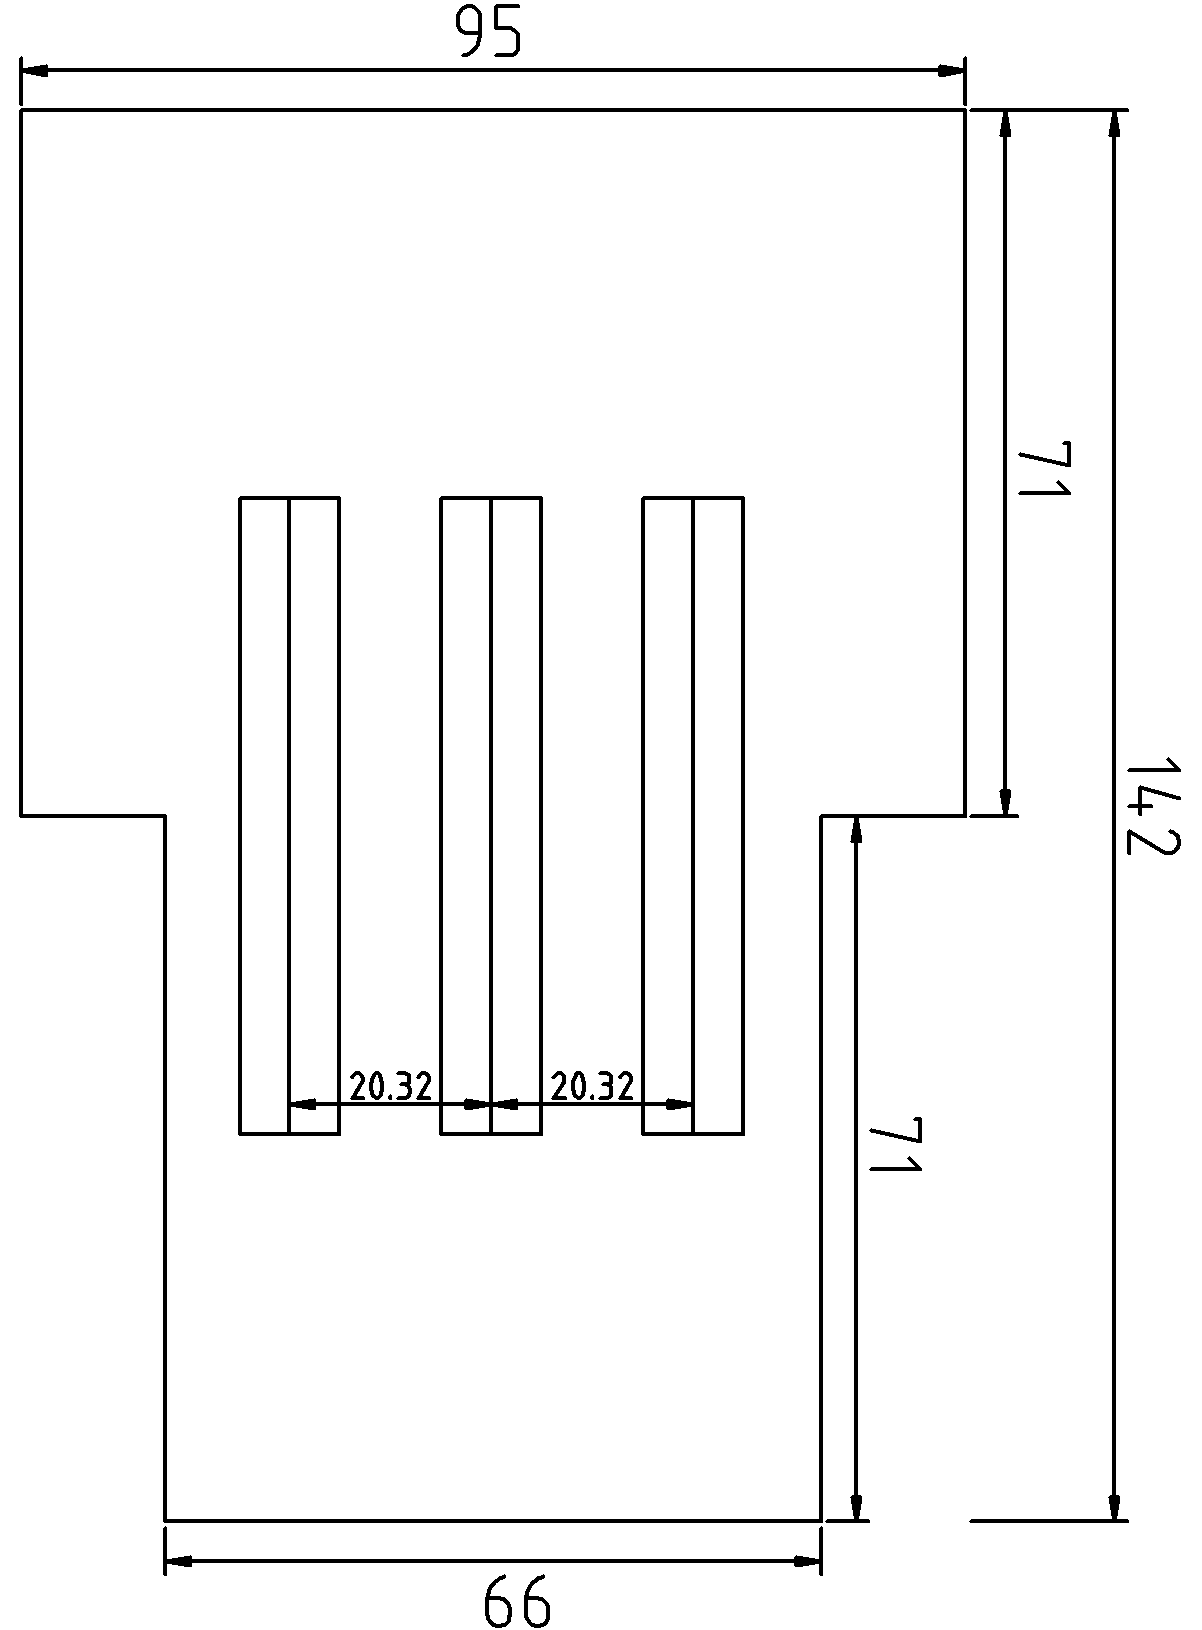
\includegraphics[width=4cm]{dim2}
		\end{minipage}
		\begin{minipage}{7cm}
			\begin{table}[ht]
				\centering
				\begin{tabularx}{.95\textwidth}{Xl}
					\textbf{Spec}			&\textbf{Value}						\\\noalign{\hrule height 2pt}
					Number of planes		&variable							\\\hline
					Interplane distance		&$20.32$\,mm						\\\hline
					Module length				&$9.5$\,cm							\\\hline
					Height					&$\approx12$\,cm					\\\hline
					Width					&$14.5$\,cm							\\\hline
					Maximum trigger area	&$7.8 \times 8$\,mm$^{2}$			\\\hline
					\multirow{2}{*}{Y-Resolution at PSI} 	&$\approx50$\,$\upmu$m for pads		\\\cline{2-2}
															&$\approx100$\,$\upmu$m	for pixel	\\\hline
				\end{tabularx}
			\end{table}
		\end{minipage}
	\end{center}
\end{frame}
% END
% ====================================================================================
% BEGIN DATATAKING
% ====================================================================================
\section{Datataking}
\begin{frame}
	\begin{alertblock}{
		\begin{center}
			\Large{\textbf{Datataking}}
		\end{center}}
	\end{alertblock}
\end{frame}
% ============================
% EUDAQ
\subsection{EUDAQ}
\begin{frame}
	\frametitle{EUDAQ}
	\underline{\textbf{Software:}}
	\begin{itemize}
		\setlength{\itemsep}{\fill}
		\item portable, modular and cross-platform DAQ framework
		\item developed for the EUDET Telescope
		\item can combine data streams from several different devices into an event based data stream
		\item utilises pXar to communicate with the telescope
		\begin{itemize}
			\item pXar-core libraries: programming and readout of the the CMS pixel chips
		\end{itemize}
	\end{itemize}
	\vspace*{.7cm}
	\underline{\textbf{Extension:}} (with guidance from DESY)
	\begin{itemize}
		\setlength{\itemsep}{\fill}
		\item readout of the analogue chip with pXar and the DTB (thanks to Simon Spannagel!)
		\item readout of diamond pad sensors with DRS4 Evaluation Board
		\item adding new class to save whole waveforms
	\end{itemize}
\end{frame}
% ============================
% TRIGGER
\subsection{Trigger}
\begin{frame}
	\frametitle{Trigger}
	\underline{\textbf{Requirements:}}\s
	\begin{itemize}
		\setlength{\itemsep}{\fill}
		\item guarantee DUT hit
		\begin{itemize}
			\item use coincidence of the fast-ORs from the planes directly before and after the DUT
		\end{itemize}
		\item scalable trigger
		\begin{itemize}
			\item mask pixels of correspondent trigger planes
		\end{itemize}
		\item exact timing
		\begin{itemize}
			\item coincidence with a fast scintillator
		\end{itemize}
		\item event alignment
		\begin{itemize}
			\item EUDAQ Trigger Logic Unit (TLU)
		\end{itemize}
	\end{itemize}
	\vspace*{.5cm}
	\underline{\textbf{Addition for pads:}}\s
	\begin{itemize}
		\item constant low frequency pulser as stable reference signal
		\begin{itemize}
			\item OR with pulser and particle trigger
		\end{itemize}
	\end{itemize}
\end{frame}
% new frame ============================
\begin{frame}
	\frametitle{Trigger Logic}
	\begin{center}
		\begin{minipage}{6cm}
			\centering
			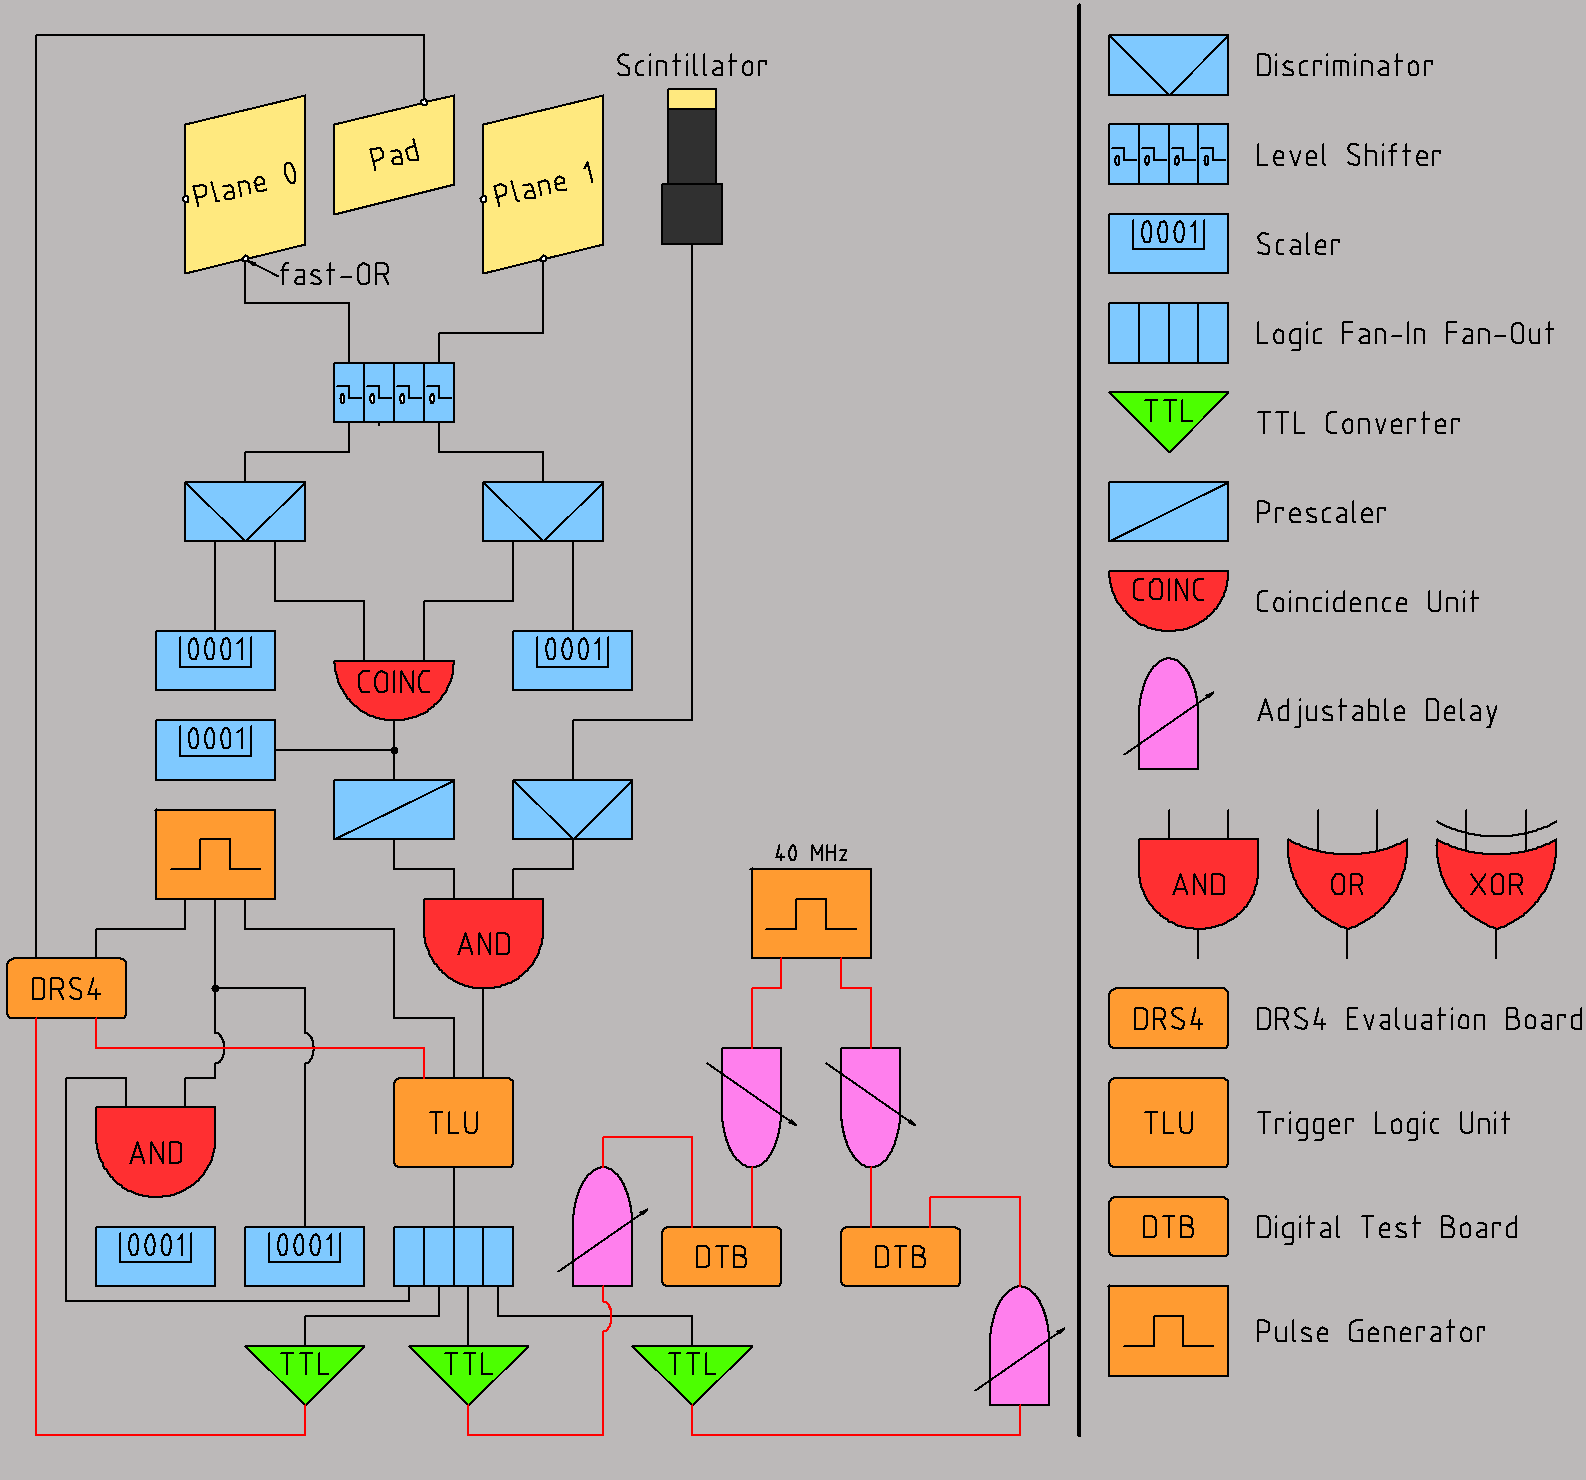
\includegraphics[width=6cm]{Pics/triglog2}
		\end{minipage}
		\hspace*{2pt}
		\begin{minipage}[c][.7\textheight]{5cm}
			\begin{itemize}
				\setlength{\itemsep}{\fill}
				\onslide<2->{\item fast-OR coincidence}
				\onslide<3->{\item coincidence with scintillator}
				\onslide<4->{\item OR with pulser}
				\onslide<5->{\item global external clock with adjustable delays}
				\onslide<6->{\item busy signal after each trigger to avoid event misalignment
				\begin{itemize}
					\item useful for events with many pixels hit 
				\end{itemize}}
			\end{itemize}
		\end{minipage}\no\s
	\end{center}
\end{frame}
% END
% ====================================================================================
% BEGIN COMMISSIONING
% ====================================================================================
\section{Commissioning}
\begin{frame}
	\begin{alertblock}{
		\begin{center}
			\Large{\textbf{Commissioning}}
		\end{center}}
	\end{alertblock}
\end{frame}
% ============================
% WBC SCAN
\subsection{WBC scan}
\begin{frame}
	\frametitle{WBC scan}
	\begin{center}
		\begin{minipage}{4.0cm}
			\centering
			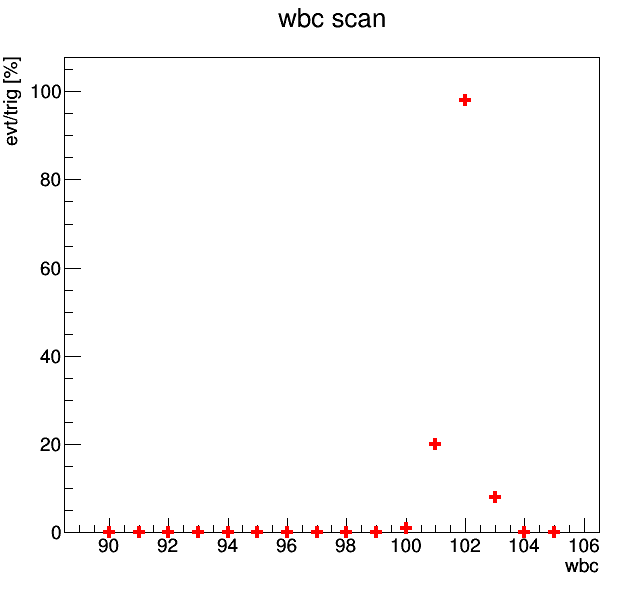
\includegraphics[width=4.0cm]{Pics/wbcscan2}
		\end{minipage}
		\hspace*{2pt}
		\begin{minipage}[c][.7\textheight]{7cm}
			\begin{itemize}
				\setlength{\itemsep}{\fill}
				\item ROC saves bunch crossing when particle hits the sensor
				\item programmable setting called wbc (wait bunch crossing)
				\item trigger only validates if time the trigger takes back to the ROC matches the wbc setting
				\item automated wbc scan using the pXar CLI
			\end{itemize}
		\end{minipage}\no\s
	\end{center}
\end{frame}
% new frame ============================
\begin{frame}
	\frametitle{Efficiency Optimisation}
	\begin{center}
		\begin{minipage}{3cm}
			\centering
			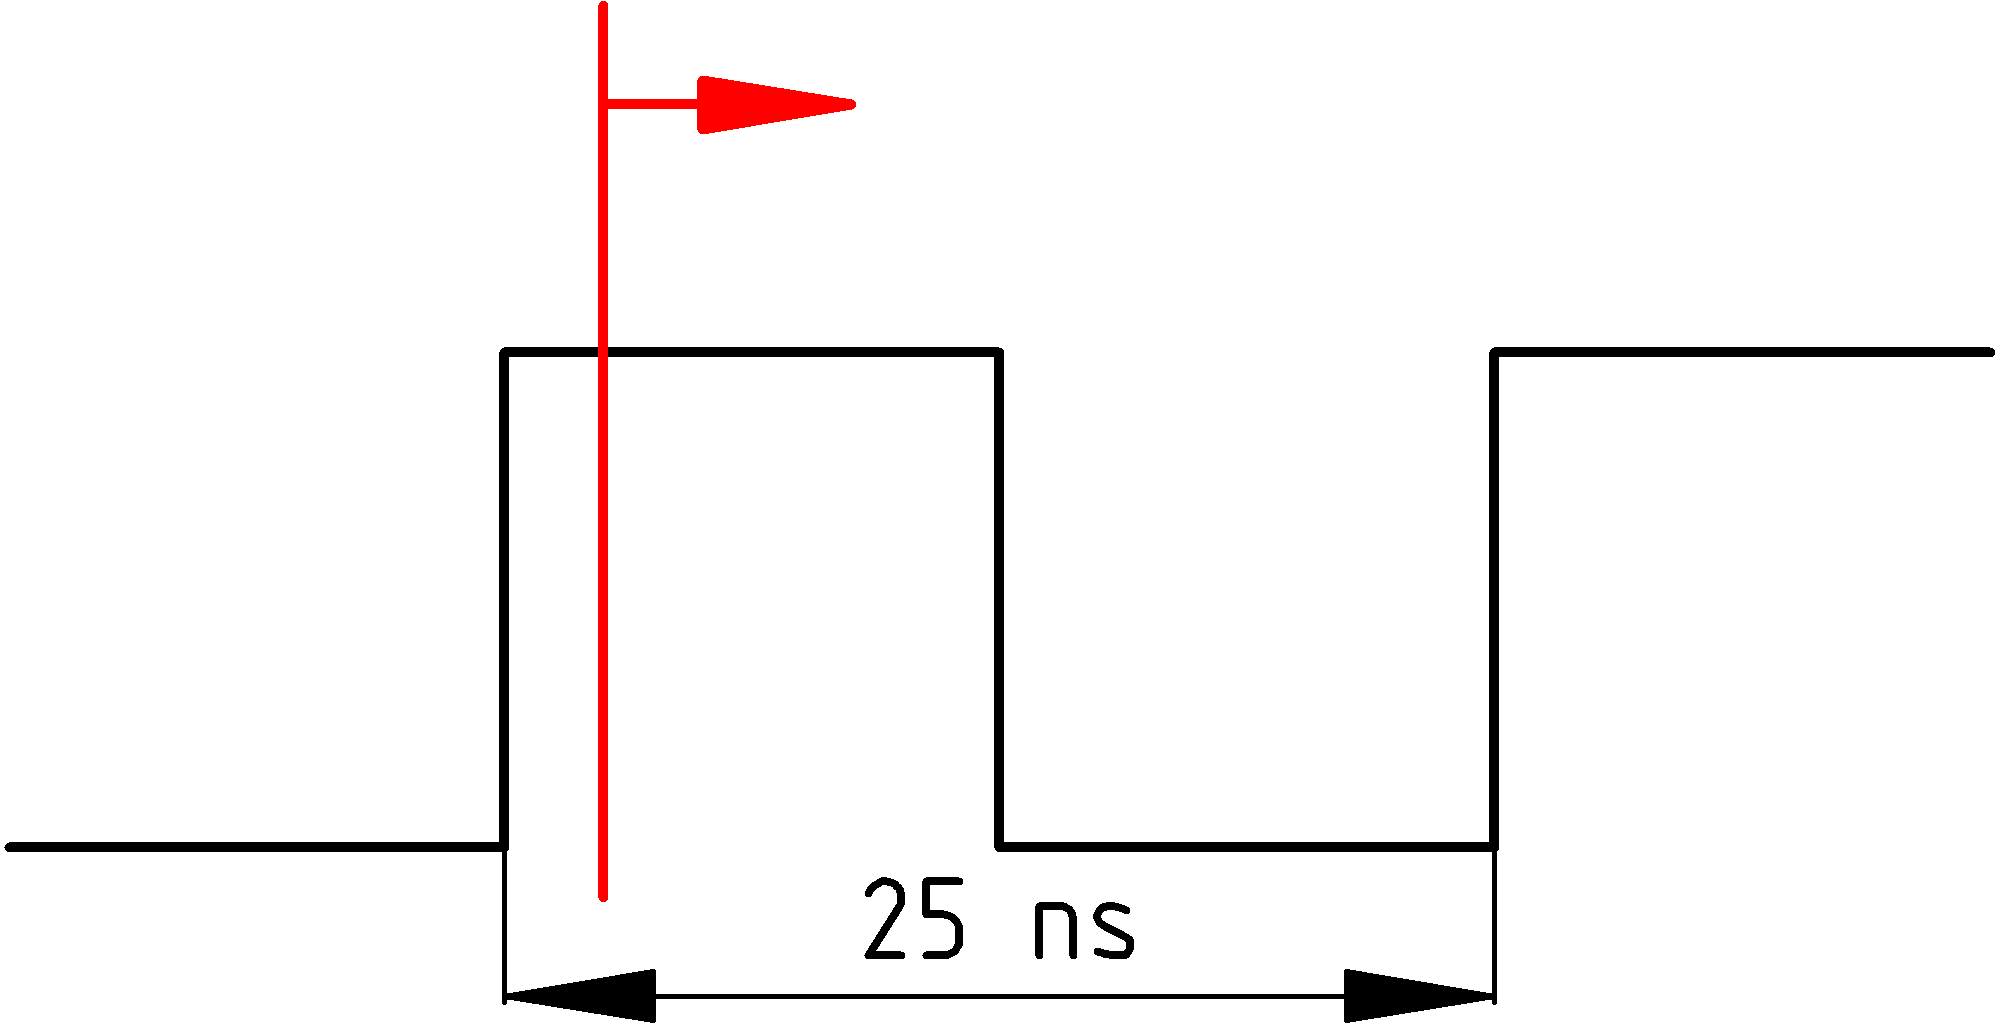
\includegraphics[width=3cm]{ClockCycle}
		\end{minipage}
		\begin{minipage}{8cm}
			\centering
			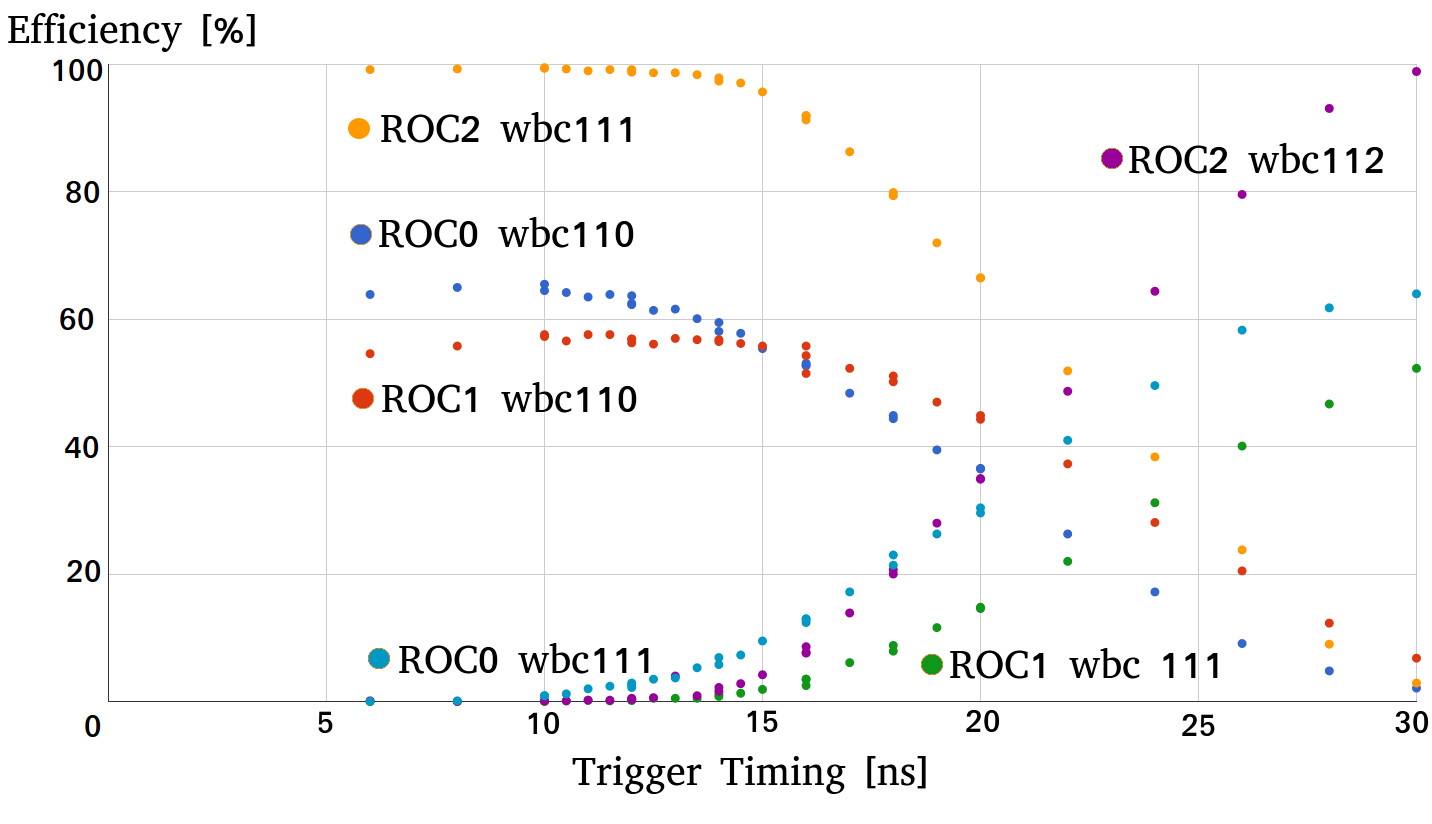
\includegraphics[height=3.5cm]{Pics/optimisation}
		\end{minipage}
	\end{center}
	\begin{itemize}
		\setlength{\itemsep}{\fill}
		\item wbc scan also yields:
			\begin{itemize}
				\item detailed information about the hit yield for every connected ROC
				\item information of the trigger phase (relative timing of the trigger compared to the clock)
			\end{itemize}
		\item first use trigger delay to shift the the trigger in the middle of the clock
		\item shift trigger and external clock delay together
		\begin{itemize}
			\item leaves trigger phase constant
			\item find optimal efficiency relative to the telescope clock
		\end{itemize}
	\end{itemize}
\end{frame}
% ============================
% ALIGNMENT
\subsection{Alignment}
\begin{frame}
	\frametitle{Event alignment}
	\begin{itemize}
		\setlength{\itemsep}{\fill}
		\item two event streams (telescope and DUT)
		\item event alignment has to be guaranteed to make use of tracking
		\item DRS4 board has no event counter
		\item using busy signal of the DRS4 as handshake for the TLU
		\item no handshake for the DTB yet (but in progress)
		\item control event alignment in online analysis
	\end{itemize}
\end{frame}
% END
% ====================================================================================
% BEGIN ANALYSIS
% ====================================================================================
\section{Analysis}
% ============================
% ALIGNMENT
\subsection{Alignment}
\begin{frame}
	\begin{alertblock}{
		\centering
		\Large{\textbf{Analysis}}}
	\end{alertblock}
	\begin{center}
		\begin{minipage}{5.5cm}
			\centering
			\begin{figure}
				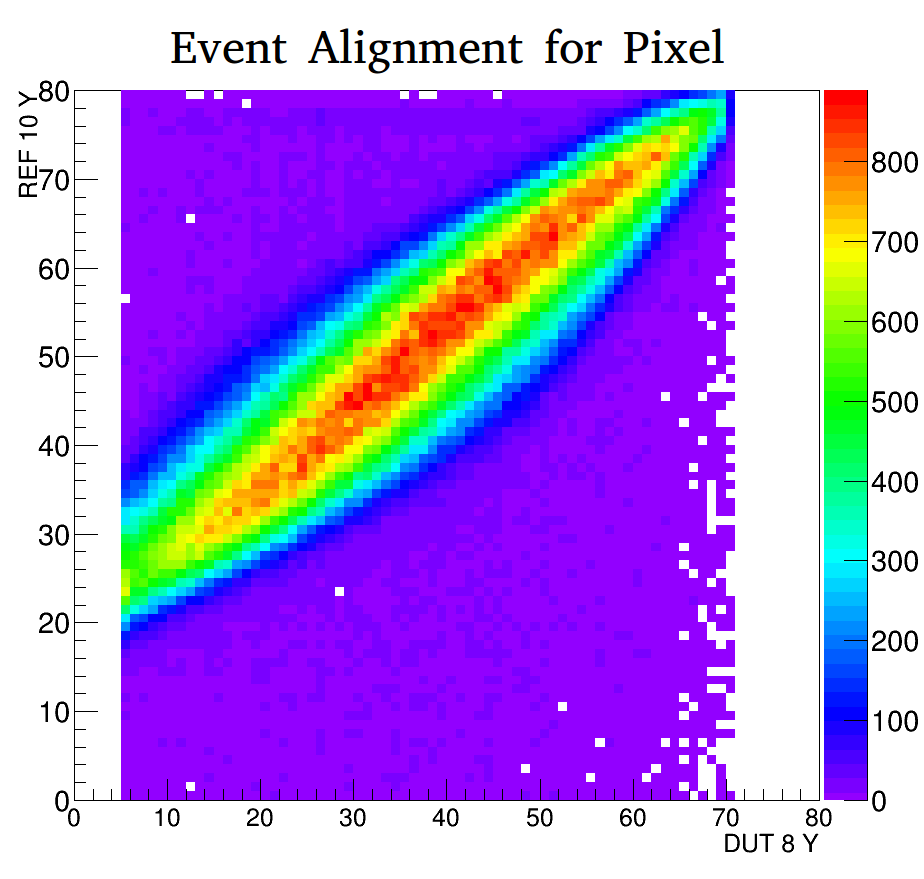
\includegraphics[width=4.4cm]{Pics/correlation2y}
			\end{figure}
			\begin{itemize}
				\item compare x and y position of telescope and DUT
			\end{itemize}
		\end{minipage}
		\hspace*{2pt}
		\begin{minipage}{5.5cm}
			\centering
			\begin{figure}
				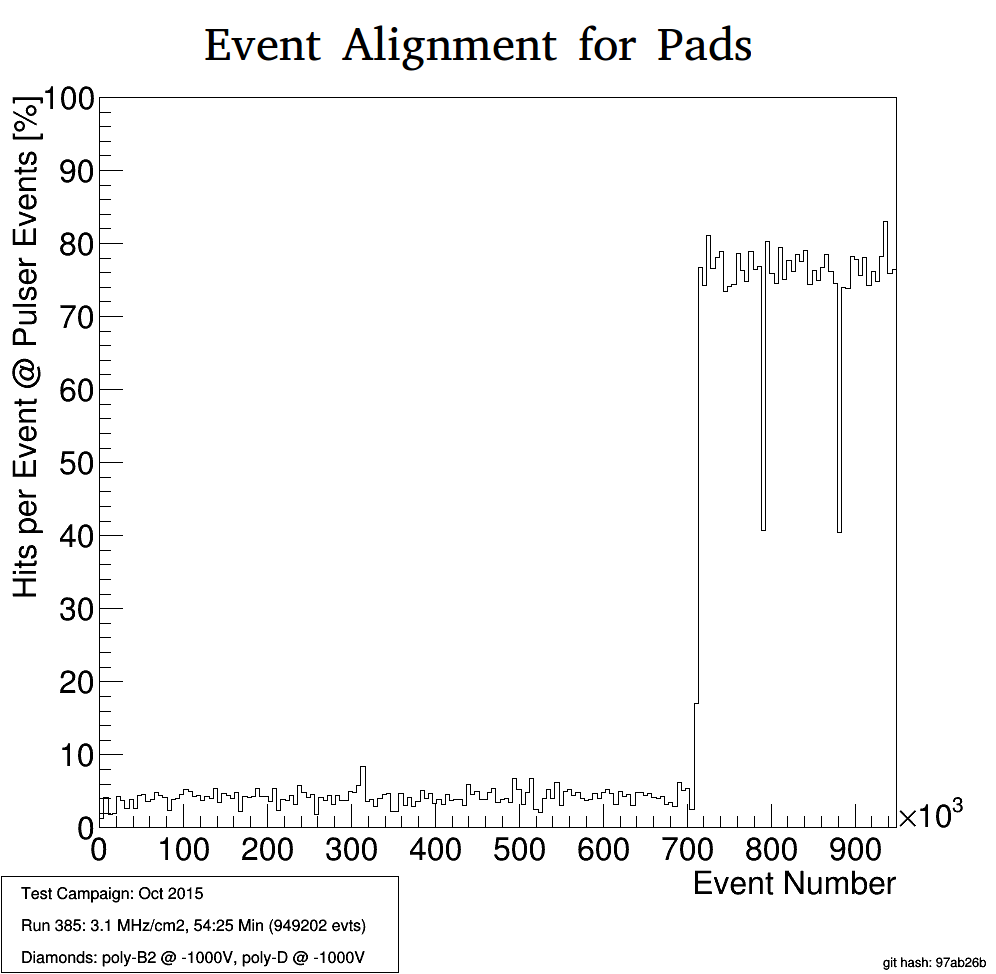
\includegraphics[width=4.4cm]{Pics/EventAlignment}
			\end{figure}
			\begin{itemize}
				\item use constant frequency pulser signal as reference
				\item expect less pixel hits at pulser events
			\end{itemize}
		\end{minipage}
	\end{center}
\end{frame}
% new frame ============================
\begin{frame}
	\frametitle{Plane alignment}
	\begin{center}
		\begin{minipage}{6cm}
			\centering
			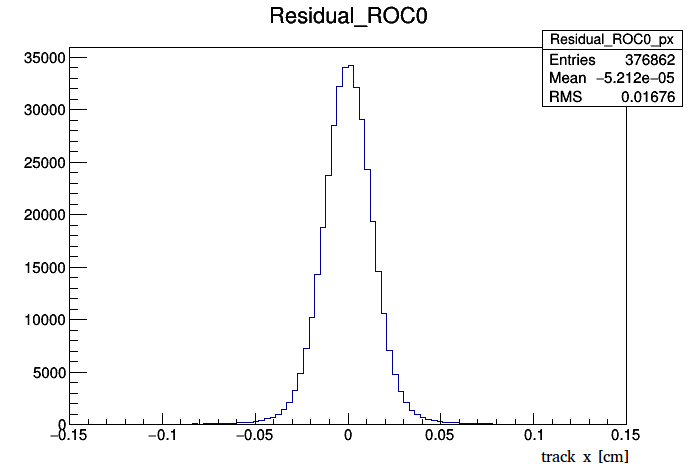
\includegraphics[width=5cm]{Residual}\\
			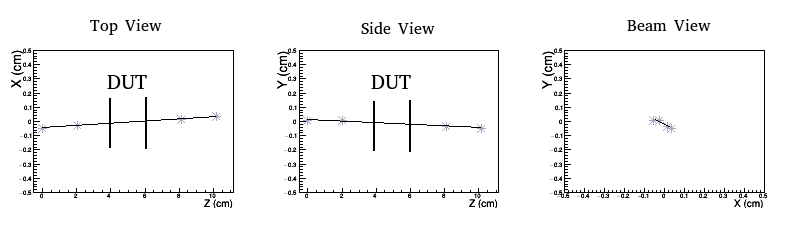
\includegraphics[width=6cm]{Track}
		\end{minipage}
		\begin{minipage}[c][.5\textheight]{5cm}
			\begin{itemize}
				\setlength{\itemsep}{\fill}
				\item iterative procedure written by Gregor Kasieczka using the PLT framework
				\item moving track residuals to zero
				\item first rotation around beam axis
				\item translation in x-y plane perpendicular to the beam axis
			\end{itemize}
		\end{minipage}
	\end{center}
\end{frame}
% ============================
% MISCELLANEOUS
\subsection{Miscellaneous}
\begin{frame}
	\begin{center}
		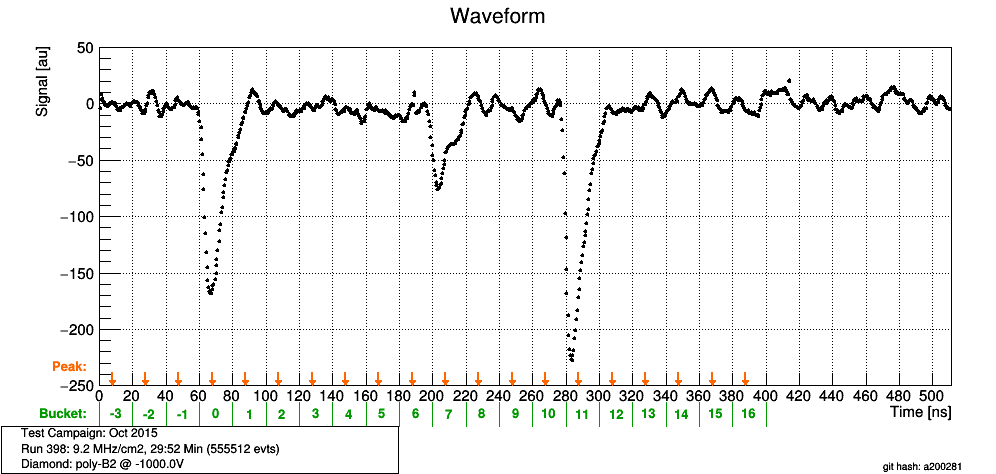
\includegraphics[width=5cm]{SingleWF}\\
		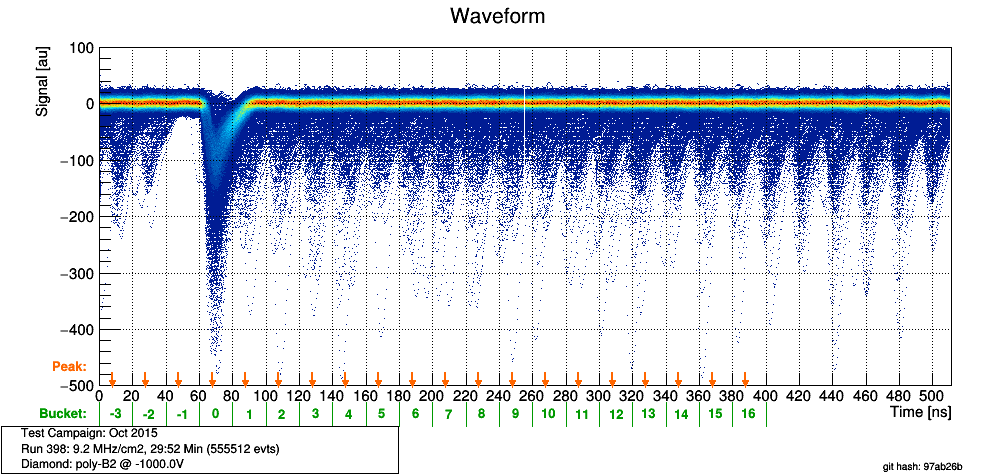
\includegraphics[width=5cm]{WaveForms5000}\\
		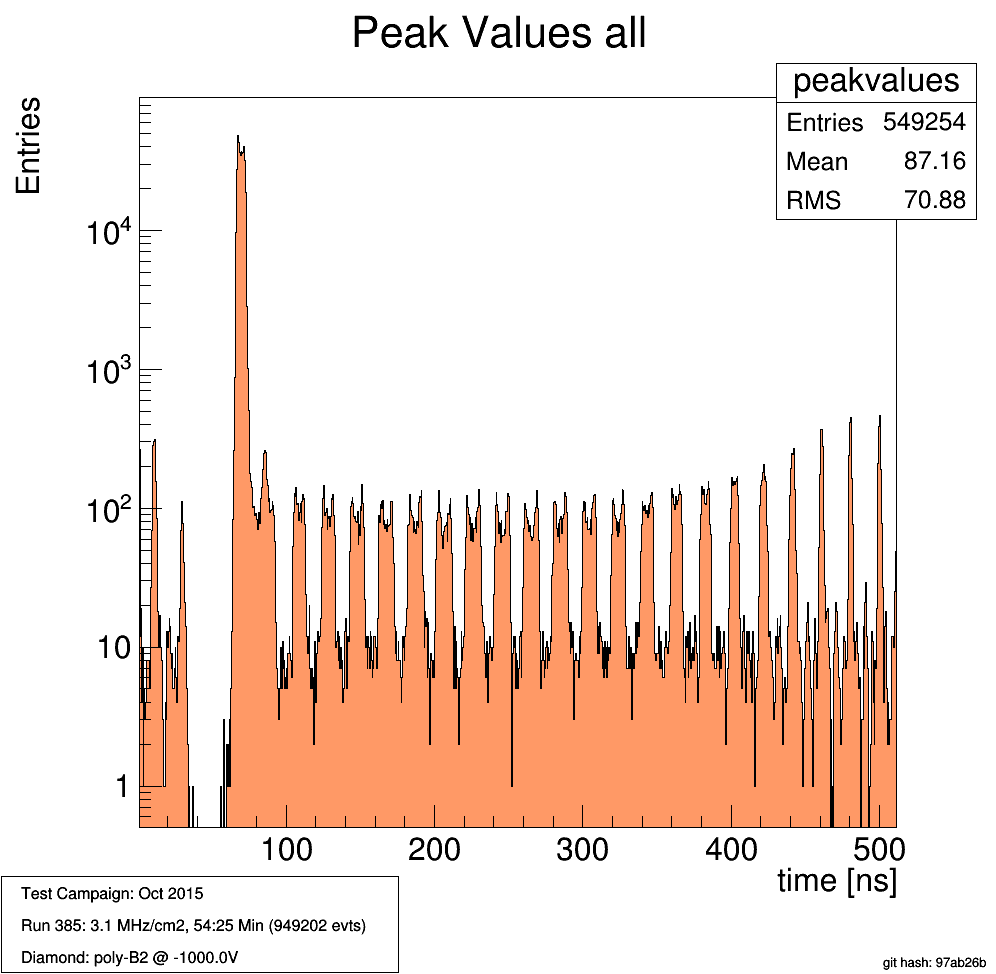
\includegraphics[width=5cm]{Pics/PeakValues}
	\end{center}
\end{frame}
% new frame ============================
\begin{frame}
	\begin{center}
		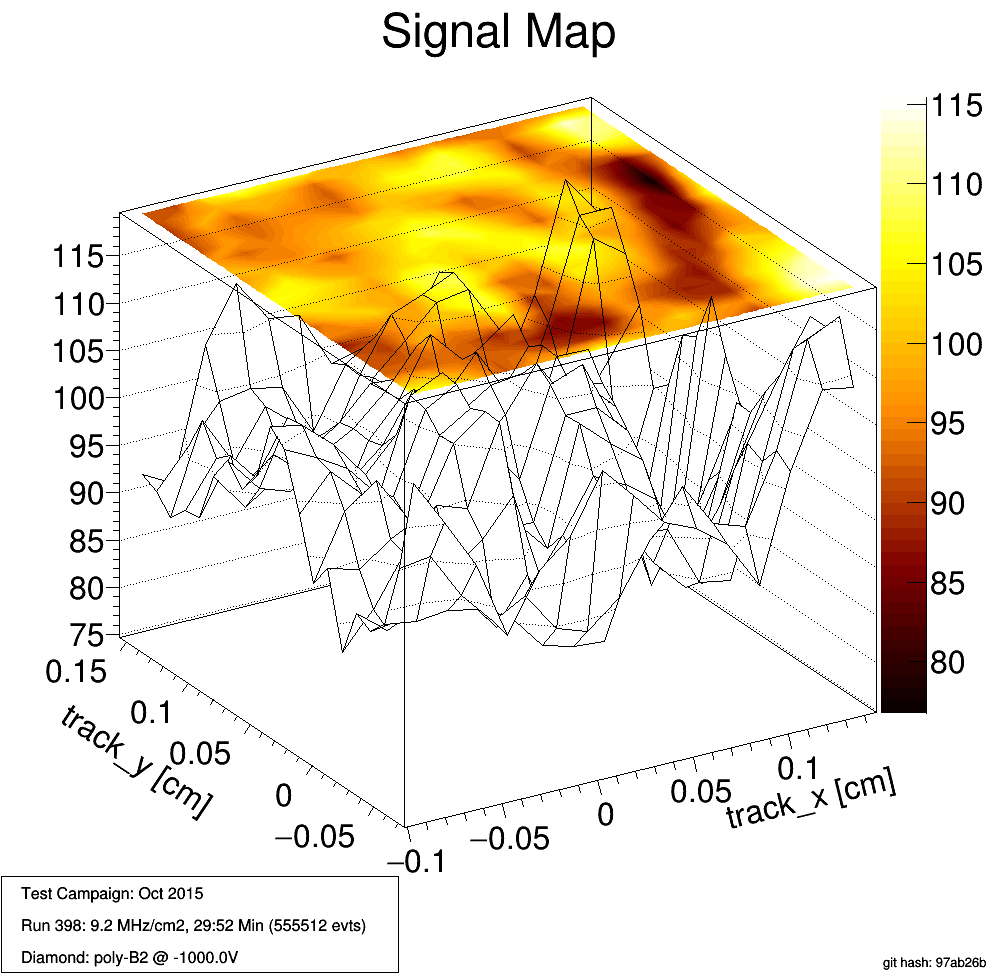
\includegraphics[width=7.0cm]{Pics/2DMap}
	\end{center}
\end{frame}

% END
% ====================================================================================
% BEGIN CONCLUSION
% ====================================================================================
\section{Conclusion}
\begin{frame}
	\begin{alertblock}{
		\begin{center}
			\Large{\textbf{Conclusion}}
		\end{center}}
	\end{alertblock}
\end{frame}
% new frame ============================
\begin{frame}
	\begin{itemize}
		\setlength{\itemsep}{\fill}
		\item overcoming problems in the beginning
		\begin{itemize}
			\item finding a good design and testing the single components
			\item readout of the analogue chip by the DTB 
			\item extending the softwares pXar and EUDAQ
		\end{itemize}
		\item great working telescope for our purposes
		\begin{itemize}
			\item reliable tracking and alignment
			\item a few runs still have event misalignment (can be fixed offline)
		\end{itemize}
		\item setup time currently about half a day
		\item still room for improvement
	\end{itemize}
\end{frame}
% END
% ====================================================================================
% BEGIN OUTLOOK
% ====================================================================================
\section{Outlook}
\begin{frame}
	\begin{alertblock}{
		\centering
		\Large{\textbf{Outlook}}}		                        
	\end{alertblock}
	\begin{itemize}
		\setlength{\itemsep}{\fill}
		\item merge trigger logic into single device (Trigger Unit)
		\begin{itemize}
			\item currently testing a TU from OSU
		\end{itemize}
		\item two preinstalled setups for pad and pixel tests
		\item synchronise DTB clock with the beam clock at PSI ($40\rightarrow50$\,MHz)
		\item save scintillator signal with the DRS4
		\begin{itemize}
			\item more precise trigger timing
			\item particle identification by time of flight
		\end{itemize}
		\item increasing resolution
		\begin{itemize}
			\item try tilting the planes (more charge sharing)
			\item reduce material
		\end{itemize}
		\item testing PROC600 as telescope chip with trigger as well as DUT
		\item testing PSI-ROC4SENS (chip without threshold) as DUT
	\end{itemize}
\end{frame}
% new frame ============================
\begin{frame}
	\underline{\textbf{Special Thanks to:}}\as
	\begin{itemize}
		\setlength{\itemsep}{\fill}
		\item the DESY people for helping us with the the EUDAQ framework
		\item Simon Spannagel for the insights in pXar and its analogue extension as well as immediate help during beam tests
		\item the Horisberger group at PSI for advice concerning the pixel chips
		\item David ... for the information about the PSI facilities
		\item $\hdots$
	\end{itemize}
\end{frame}
% END
% ====================================================================================
% BEGIN BACKUP
% ====================================================================================
\section*{Backup}
% ============================
% MOTHERBOARD
\subsection*{Telescope Parts}
\begin{frame}
	\addtocounter{framenumber}{-1}
	\frametitle{Motherboard}
	\begin{center}
		\begin{minipage}{4.6cm}
			\centering
			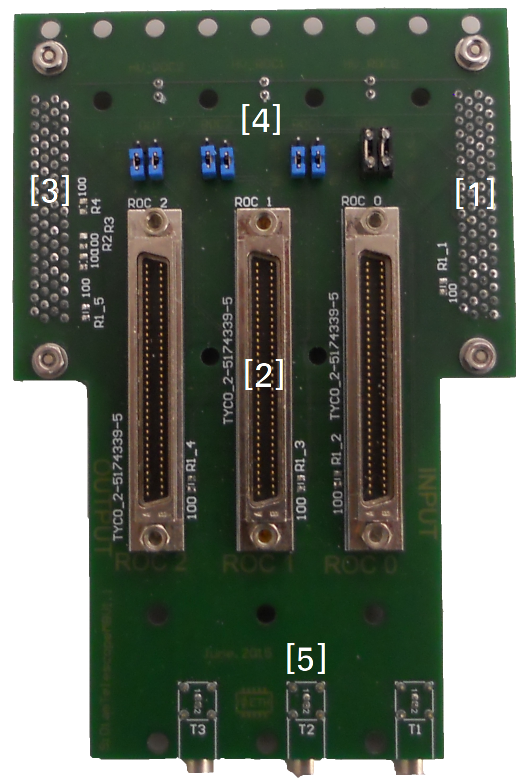
\includegraphics[width=4.35cm]{Pics/Motherboard}
		\end{minipage}
		\hspace*{2pt}
		\begin{minipage}[c][.7\textheight]{6cm}
			\begin{itemize}
				\setlength{\itemsep}{\fill}
				\item $[1]$ input: SCSI connector to the DTB
				\item $[2]$ sockets for the adapter planes
				\item $[3]$ output (optional): SCSI connector to another motherboard
				\begin{itemize}
					\item daisy-chainable
				\end{itemize}
				\item $[4]$ token jumpers:
				\begin{itemize}
					\item blue\hspace{4pt} = plane used
					\item black = plane skipped
				\end{itemize}
				\item $[5]$ output of the fast-OR trigger signal 
			\end{itemize}
		\end{minipage}\no\s
	\end{center}
\end{frame}
% ============================
% PLANES
\begin{frame}
	\addtocounter{framenumber}{-1}
	\frametitle{Adapter Planes}
	\begin{center}
		\begin{minipage}{4cm}
			\centering
			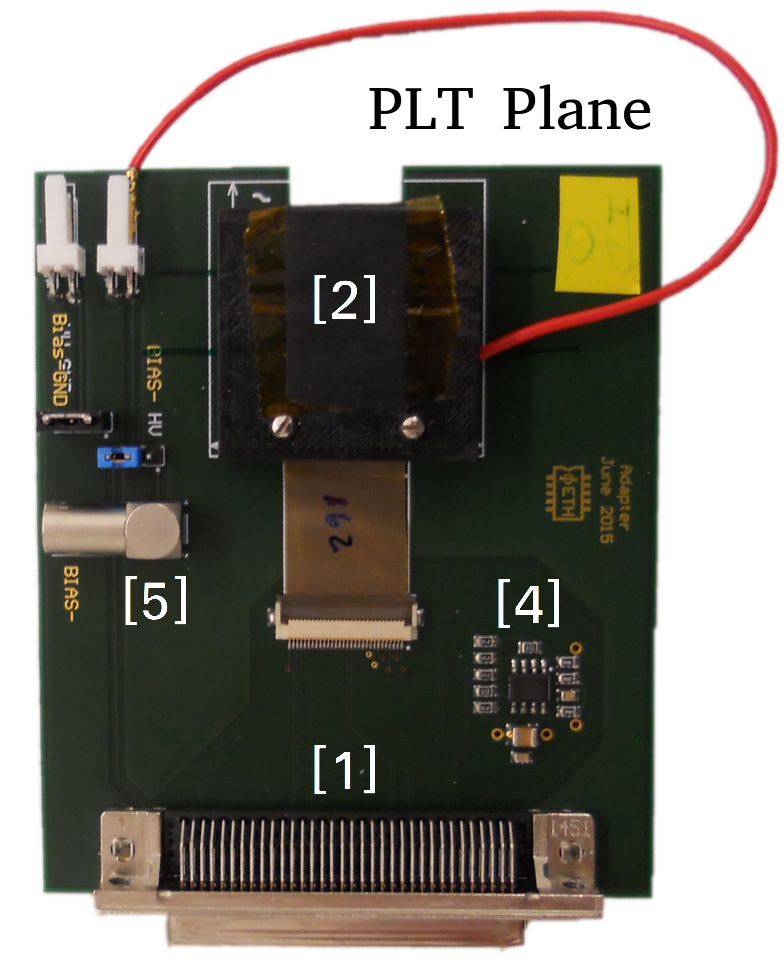
\includegraphics[width=3.4cm]{Pics/AdapterAnalog}
		\end{minipage}
		\hspace*{2pt}
		\begin{minipage}{7cm}
			\centering
			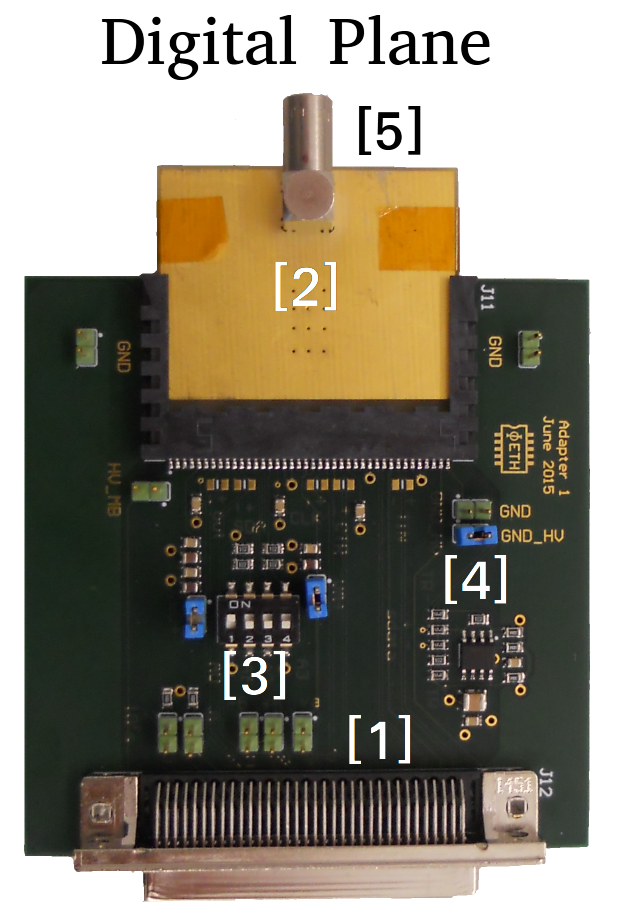
\includegraphics[width=5.6cm]{Pics/AdapterDigital}
		\end{minipage}
	\end{center}
	\begin{center}
		\begin{minipage}{5.5cm}
			\begin{itemize}
				\item $[1]$ SCSI connector to MB
				\item $[2]$ CMS pixel chip
				\item $[3]$ bit switch for I$^{2}$C address
			\end{itemize}
		\end{minipage}
		\hspace*{2pt}
		\begin{minipage}{5.5cm}
			\begin{itemize}
				\item $[4]$ fast-OR amplifying circuit
				\item $[5]$ sensor bias input
			\end{itemize}
		\end{minipage}
	\end{center}
\end{frame}
% ============================
% ANALOGUE CHIP
\subsection{Inclusion of the analogue pixel chip}
\begin{frame}
	\addtocounter{framenumber}{-1}
	\frametitle{Inclusion of the analogue pixel chip}
	\begin{itemize}
		\setlength{\itemsep}{\fill}
		\item analogue chips were read out with an Analogue Test Board (ATB)
		\begin{itemize}
			\item limited buffer size ($\rightarrow$ limited run time)
		\end{itemize}
		\item adapting pXar to use the DTB for the readout (thanks to Simon Spannagel)
		\item need to adjust DTB timings:
		\begin{itemize}
			\item token delays to find the begin and the end of the waveform
			\item clock offset to sample at the center of each peak of the waveform
		\end{itemize}
	\end{itemize}
	\begin{center}
		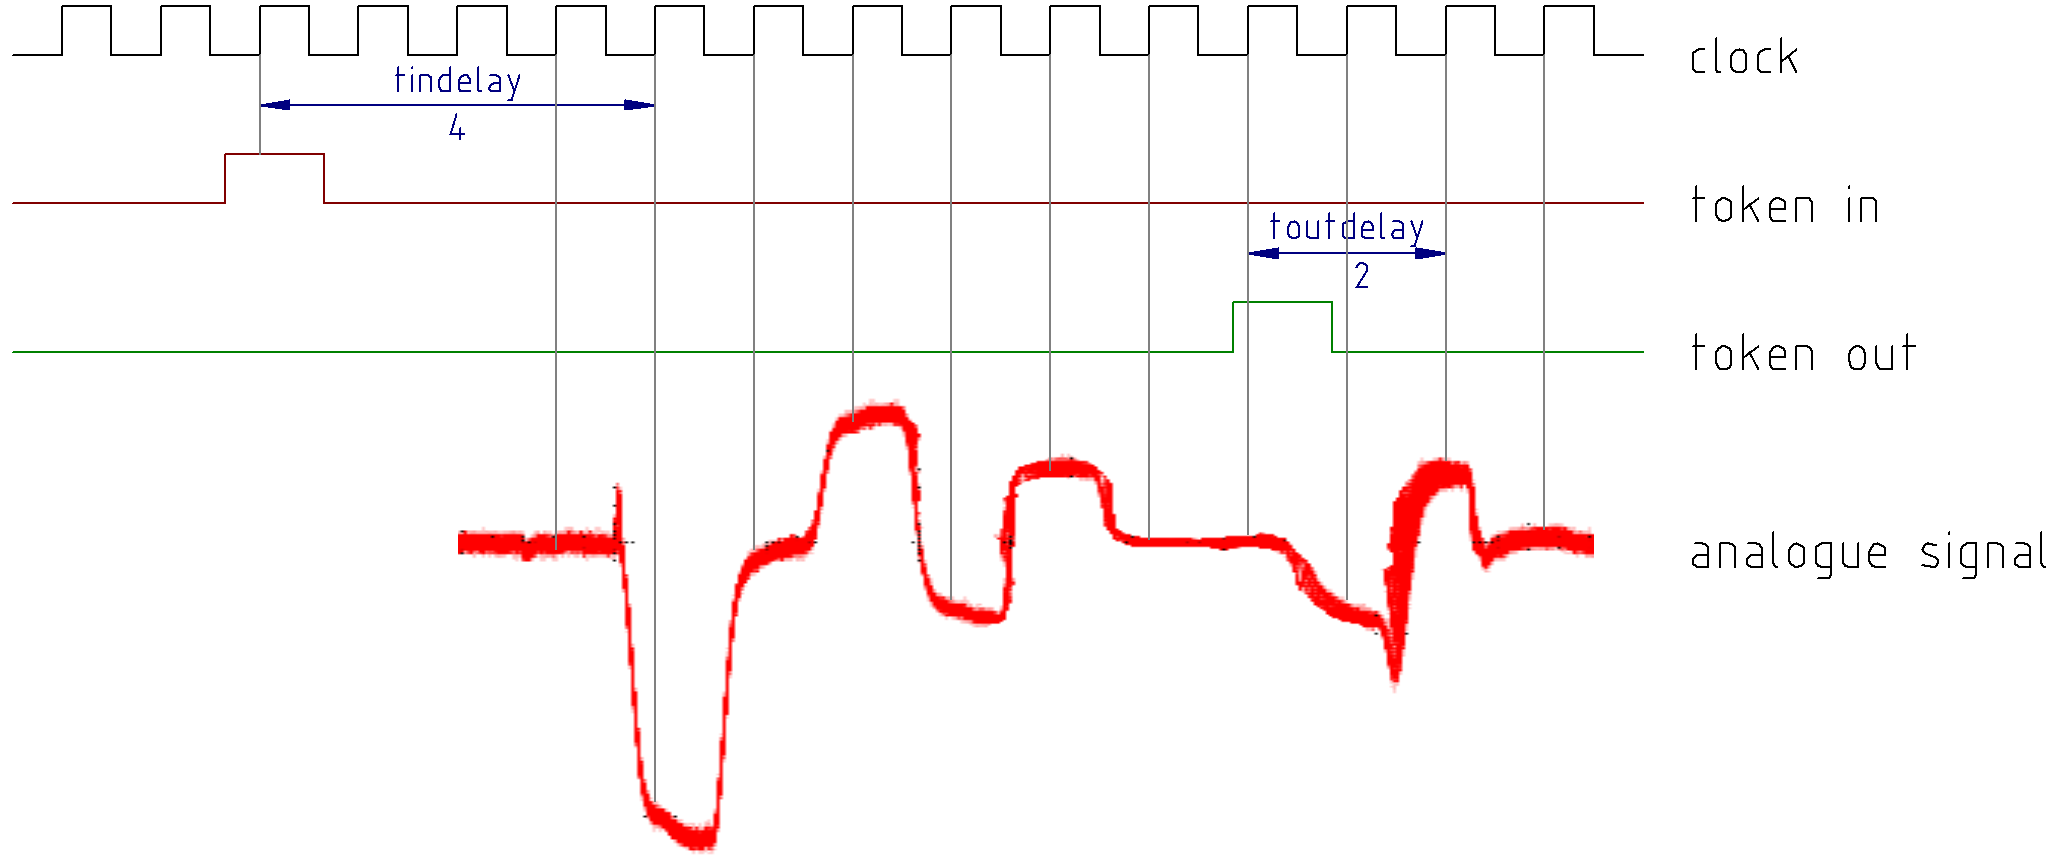
\includegraphics[width=8cm]{tbdelays}
	\end{center}
\end{frame}
% ============================
% THE DIGITAL TESTBOARD
\subsection*{The DTB}
\begin{frame}
	\addtocounter{framenumber}{-1}
	\frametitle{The Digital Test-Board}
	\begin{itemize}
		\setlength{\itemsep}{\fill}
		\item FPGA including soft Token Bit Manager (TBM) emulator
		\item clock and external trigger inputs
		\item connectors: USB, low voltage and scsi 
		\item LEMO high voltage input for biasing the sensors
		\item internal ADC
	\end{itemize}
	\begin{center}
		\begin{minipage}{5cm}
			\centering
			\begin{figure}
				\caption{DTB inside}
				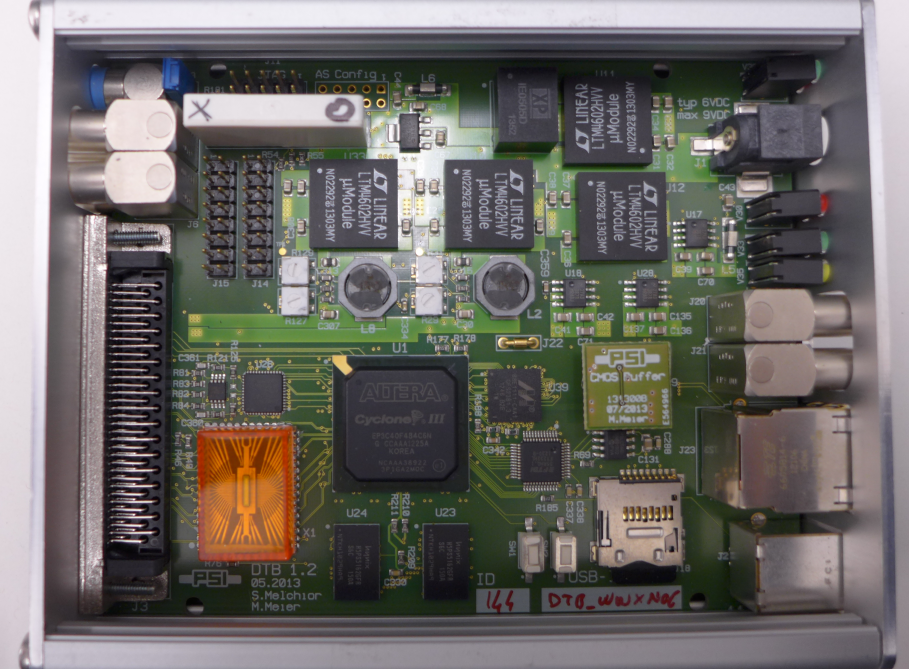
\includegraphics[width=4.5cm]{Pics/dtb_inside}
			\end{figure}
		\end{minipage}
		\hspace*{2pt}
		\begin{minipage}{5cm}
			\centering
			\begin{figure}
				\caption{DTB front and back}
				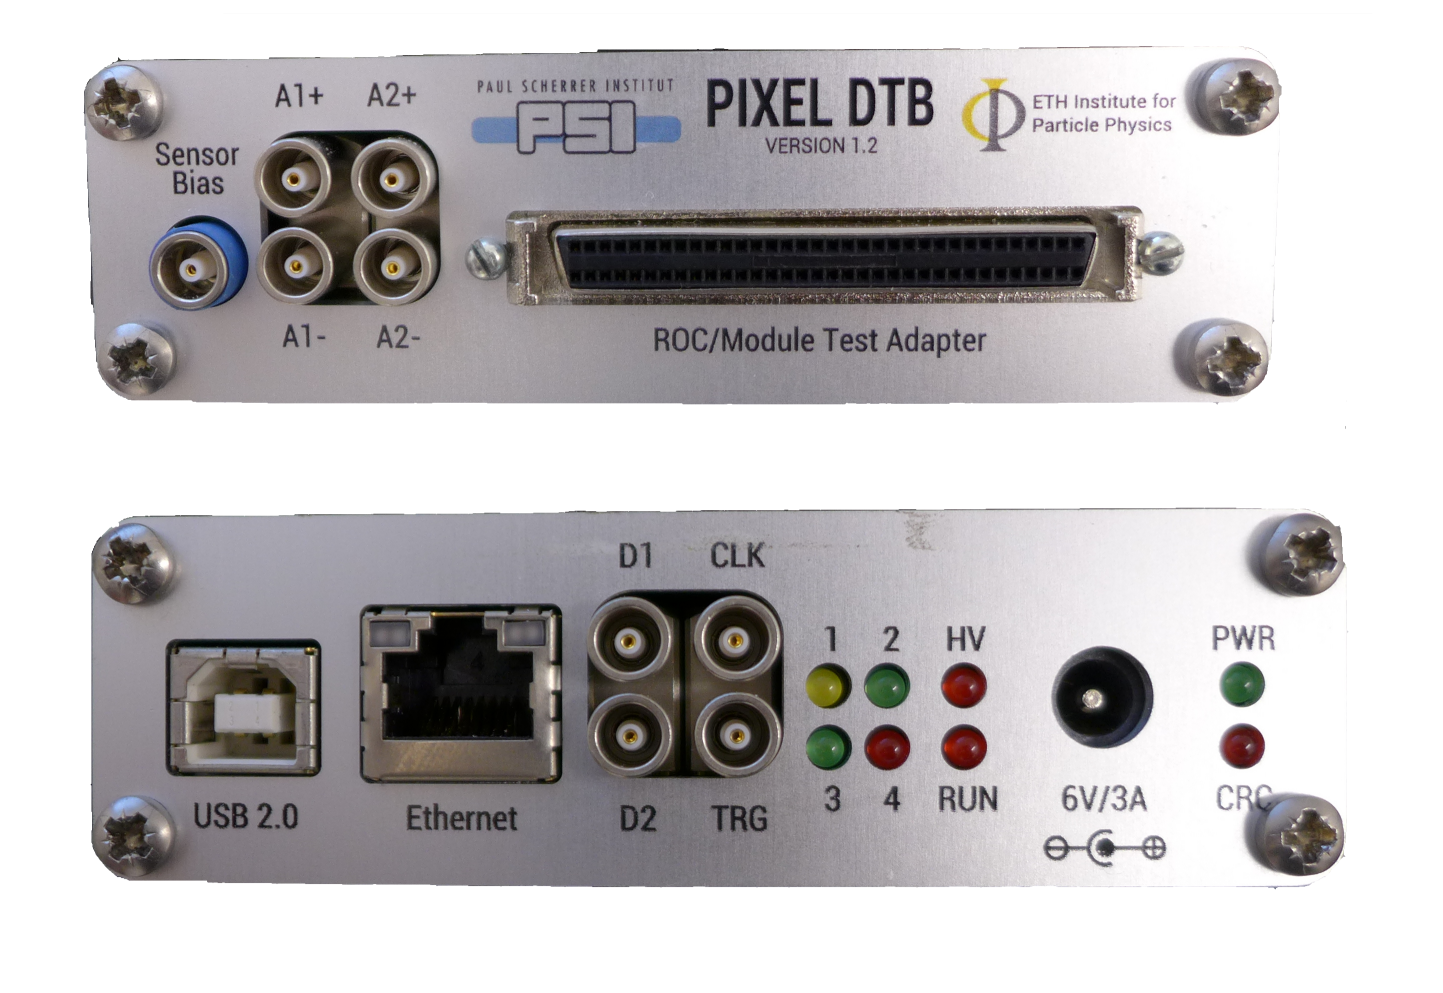
\includegraphics[width=4.5cm]{Pics/DTB-Sides}
			\end{figure}
		\end{minipage}\no\s
	\end{center}
\end{frame}
% END
% ============================
% DOCUMENT END
\end{document}

